\documentclass[a4paper, 12pt]{article}

\usepackage{minted}
\usepackage{secdot}
\usepackage{cmap}
\usepackage[utf8]{inputenc}
\usepackage[english,russian]{babel}
\usepackage[a4paper, left=3cm, right=1.5cm, top=2cm, bottom=2cm]{geometry}
\usepackage{setspace}
\usepackage{tikz}
\usepackage{adjustbox}
\usepackage{titlesec}
\usepackage{ifthen}
\usepackage{color}
\usepackage{amsmath}
\usepackage{mathtools}
\usepackage{listings}
\usepackage{hyphenat}
\usepackage{amssymb} % для \mathbb{N}
\usepackage[ruled,vlined]{algorithm2e} % Параметры: ruled — с линейкой, vlined — вертикальные линии

% График (barchart)
\usepackage{pgfplots}
\pgfplotsset{compat=1.18}
\usepackage[T2A]{fontenc}  % Изменили на T2A для правильной поддержки кириллицы
\usepackage{cmap}          % Для улучшенного поиска в PDF
\usepackage{mathtext}      % Для правильного отображения математических символов в кириллице

\usepackage[unicode, pdftex]{hyperref}
\usepackage{csquotes}
\usepackage[
    style=gost-numeric,
    language=auto,
    autolang=other
]{biblatex}

% Настройка стиля листинга
\lstset{
    language=C++,
    basicstyle=\ttfamily\small,
    breaklines=true,
    frame=single,
    inputencoding=utf8,
    extendedchars=true,
    keepspaces=true,
    showstringspaces=false,
    numbers=left, % Нумерация строк
    numberstyle=\tiny\color{gray},
    rulecolor=\color{black},
    captionpos=b, % Подпись снизу
    belowcaptionskip=5pt,
    literate={% Полная таблица замен для кириллицы
        а}{{\cyra}}1 {б}{{\cyrb}}1 {в}{{\cyrv}}1 {г}{{\cyrg}}1 {д}{{\cyrd}}1
        {е}{{\cyre}}1 {ё}{{\cyryo}}1 {ж}{{\cyrzh}}1 {з}{{\cyrz}}1 {и}{{\cyri}}1
        {й}{{\cyrishrt}}1 {к}{{\cyrk}}1 {л}{{\cyrl}}1 {м}{{\cyrm}}1 {н}{{\cyrn}}1
        {о}{{\cyro}}1 {п}{{\cyrp}}1 {р}{{\cyrr}}1 {с}{{\cyrs}}1 {т}{{\cyrt}}1
        {у}{{\cyru}}1 {ф}{{\cyrf}}1 {х}{{\cyrh}}1 {ц}{{\cyrc}}1 {ч}{{\cyrch}}1
        {ш}{{\cyrsh}}1 {щ}{{\cyrshch}}1 {ъ}{{\cyrhrdsn}}1 {ы}{{\cyrery}}1
        {ь}{{\cyrsftsn}}1 {э}{{\cyrerev}}1 {ю}{{\cyryu}}1 {я}{{\cyrya}}1
        {А}{{\CYRA}}1 {Б}{{\CYRB}}1 {В}{{\CYRV}}1 {Г}{{\CYRG}}1 {Д}{{\CYRD}}1
        {Е}{{\CYRE}}1 {Ё}{{\CYRYO}}1 {Ж}{{\CYRZH}}1 {З}{{\CYRZ}}1 {И}{{\CYRI}}1
        {Й}{{\CYRISHRT}}1 {К}{{\CYRK}}1 {Л}{{\CYRL}}1 {М}{{\CYRM}}1 {Н}{{\CYRN}}1
        {О}{{\CYRO}}1 {П}{{\CYRP}}1 {Р}{{\CYRR}}1 {С}{{\CYRS}}1 {Т}{{\CYRT}}1
        {У}{{\CYRU}}1 {Ф}{{\CYRF}}1 {Х}{{\CYRH}}1 {Ц}{{\CYRC}}1 {Ч}{{\CYRCH}}1
        {Ш}{{\CYRSH}}1 {Щ}{{\CYRSHCH}}1 {Ъ}{{\CYRHRDSN}}1 {Ы}{{\CYRERY}}1
        {Ь}{{\CYRSFTSN}}1 {Э}{{\CYREREV}}1 {Ю}{{\CYRYU}}1 {Я}{{\CYRYA}}1
}

\DeclarePairedDelimiter{\ceil}{\lceil}{\rceil}

\linespread{1.4}

\addbibresource{src/references.bib}

\begin{document}

	\begin{titlepage}
	\begin{center}
	{\bf Федеральное государственное автономное образовательное учреждение \\
	высшего образования \\
	Московский физико-технический институт                                      \\
	(национальный исследовательский университет) \\ }
	Физтех-школа радиотехники и компьютерных технологий \\
	Кафедра системного программирования \\
	\vspace{1em}
	\end{center}

	\begin{center}
	\vspace{1cm}

	\vspace{\fill}

	\begin{LARGE}
	Разработка высокопроизводительных библиотек машинного обучения в графических процессорах общего назначения \\
	\end{LARGE}
	\vspace{1em}
	% Бакалаврская работа
	\vspace{1.5cm}
	\vspace{\fill}
	\end{center}


	\begin{flushright}
	Обучающийся\\
	Штром Кристофер Дезидерович\\

	\vspace{2em}
	Научный консультант \\
	Маслов Максим Владимирович\\

	\vspace{2em}
	Научный руководитель \\
	Морозов Сергей Вячеславович\\

	\end{flushright}

	\vspace{7em}

	\begin{center}
	Москва
	\the\year{}
	\end{center}
\end{titlepage}


	\tableofcontents
	\clearpage

	\section{Введение}
Графический процессор общего назначения (далее GPGPU - general-purpose graphics processing unit) является доминирующим решением
в задачах машинного обучения. Технологии машинного обучения требуют большого количества вычислительных ресурсов и обладают высокой
степенью параллельности. Графические процессоры изначально были созданы для обработки большого количества независимых данных
(например, набора пикселей), поэтому обладают необходимой степенью параллельности и соответствуют вычислительным требованиям
методов машинного обучения.

Индустриальным стандартом GPGPU являются графические процессоры компании Nvidia \cite{nvidia_2025}. Лидирующее положение Nvidia в области
ускорителей для искусственного интеллекта является следствием не только высокой производительности аппаратных решение, но также
развитой системы программного обеспечения. Среди программного стека Nvidia наиболее важными частями являются:
\begin{itemize}
    \item Программно-аппаратная модель CUDA \cite{cuda_guide_2025}
    \item Специализированные оптимизированные библиотеки, такие как:
    \begin{itemize}
        \item cuBLAS \cite{cublas_2025} — для операций линейной алгебры
        \item cuDNN \cite{cudnn_2025} — для операций свертки, пакетной нормализации и т.д.
    \end{itemize}
    \item интеграция с популярными фреймворками машинного обучения, такими как \\
          PyTorch \cite{pytorch_2025} и TensorFlow \cite{tensorflow_2025}
\end{itemize}
Такая сильно развитая система программного обеспечения позволяет разработчикам использовать эффективные инструменты для реализации задач машинного
обучения на GPGPU.

При разработке конкурентноспособных решений в области GPGPU необходимо уделить особое внимание разработке эффективных
программных инструментов и библиотек, а также обеспечить совместимость с существующими фреймворками машинного обучения.
Помимо достижения высокой производительности, это обеспечит плавный переход разработчиков на новую платформу.

Настоящая дипломная работа посвящена разработке высокопроизводительных библиотек машинного обучения, предназначенных для работы на GPGPU, поддерживающую
программно-аппаратную модель CUDA. В качестве исследовательской базы используется функциональный и потактовый симулятор графического процессора,
поддерживающий модель CUDA, на основе симулятора компьютерных систем gem5 \cite{gem5_2025}. Основное внимание уделено разработке специализированных библиотек:
линейной алгебры cuBLAS и нейронных сетей cuDNN, а также адаптации этих инструментов для совместимости c фреймворком машинного обучения PyTorch.
Симулятор вместе с программным обеспечением, включающая в себе драйвер симулируемого графического процессора и библиотеку среды выполнения CUDA позволяет
запускать CUDA-программы. Ввиду значительных ограничений производительности программной симуляции графического процессора, исследование
производительности было проведено на реальных графических процессорах Nvidia: Tesla V100 \cite{tesla_v100_2025} и Jetson Xavier \cite{jetson_xavier_2025}.

Специализированные библиотеки, такие как cuBLAS и cuDNN имеют решающее значение при разработке программного обеспечения, необходимого для успешной
работы задач машинного обучения на GPGPU, поэтому исследование этих инструментов стало основным. В ходе исследования были выбраны наиболее критически
важные интерфейсы библиотек cuBLAS и cuDNN:
\begin{itemize}
    \item \texttt{cublasLtMatmul} — общее матричное умножение (GEMM — general matrix multiplic\-ation)
    \item \texttt{cudnnConvolutionForward} — прямая свертка тензора (обычно 4-мерного в формате NCHW или NHWC)
    \item \texttt{cudnnBatchNormalizationForwardInference} — пакетная нормализация тензора
\end{itemize}
Ввиду того, что библиотеки cuBLAS и cuDNN являются проприетарными решениями, необходима собственная реализация этих интерфейсов.
Данные интерфейсы были разработаны, и было проведено исследование их производительности на графических процессорах Nvidia. Реализации данных интерфейсов
активно задействуют библиотеку CUTLASS \cite{cutlass_2025}, представляющую собой высокопроизводительную коллекцию шаблонов и компонентов для линейной алгебры
на CUDA и являющаяся проектом с открытым исходным кодом. Основными преимущества CUTLASS являются:
\begin{itemize}
    \item Возможность переиспользования частей высокопроизводительных алгоритмов
    \item Настройка параметров алгоритмов
    \item Поддержка различных типов данных
\end{itemize}

Для верификации корректности работы реализованных интерфейсов была проведена серия экспериментов по запуску реальных нейронных сетей с использованием фреймворка PyTorch.
Тестирование включало:
\begin{itemize}
    \item Сравнение результатов вычислений с эталонными реализациями
    \item Замеры производительности на различных типах нейронных сетей
    \item Анализ масштабируемости при работе с тензорами разных размеров и форматов
\end{itemize}

Были получены результаты, демонстрирующие работоспособность предложенных реализаций и их соответствие требованиям высокой производительности.
	\clearpage

	\section{Постановка задачи}
\subsection{Цель работы}
\begin{enumerate}
\item Разработать высокопроизводительные библиотеки машинного обучения cuBLAS и cuDNN для запуска матричного умножения,
операции свертки и пакетной нормализации и провести запуск на функциональном и потактовом симуляторе, поддерживающего
программно-аппаратную модель CUDA
\item Проверить работоспособность и производительность разработанных библиотек на нейронных сетях, использующих фреймворк
машинного обучения PyTorch
\end{enumerate}

\subsection{Задачи}
Задачи, которые необходимо решить в рамках данной работы:
\begin{enumerate}
\item Разработать интерфейсы матричного умножения, операции свертки и пакетной нормализации из библиотеки cuBLAS и cuDNN
\item Определить методологию тестирования и проверить работоспособность разработанных интерфейсов на нейронных сетях,
использующих фреймворк PyTorch
\item Провести исследование масштабируемости интерфейсов на разные форматы и типы данных
\item Определить методологию измерения производительности интерфейсов и провести анализ производительности
\end{enumerate}
	\clearpage

	\section{Используемые технологии}
\subsection{Модель CUDA}
\begin{figure}[h]
    \centering
    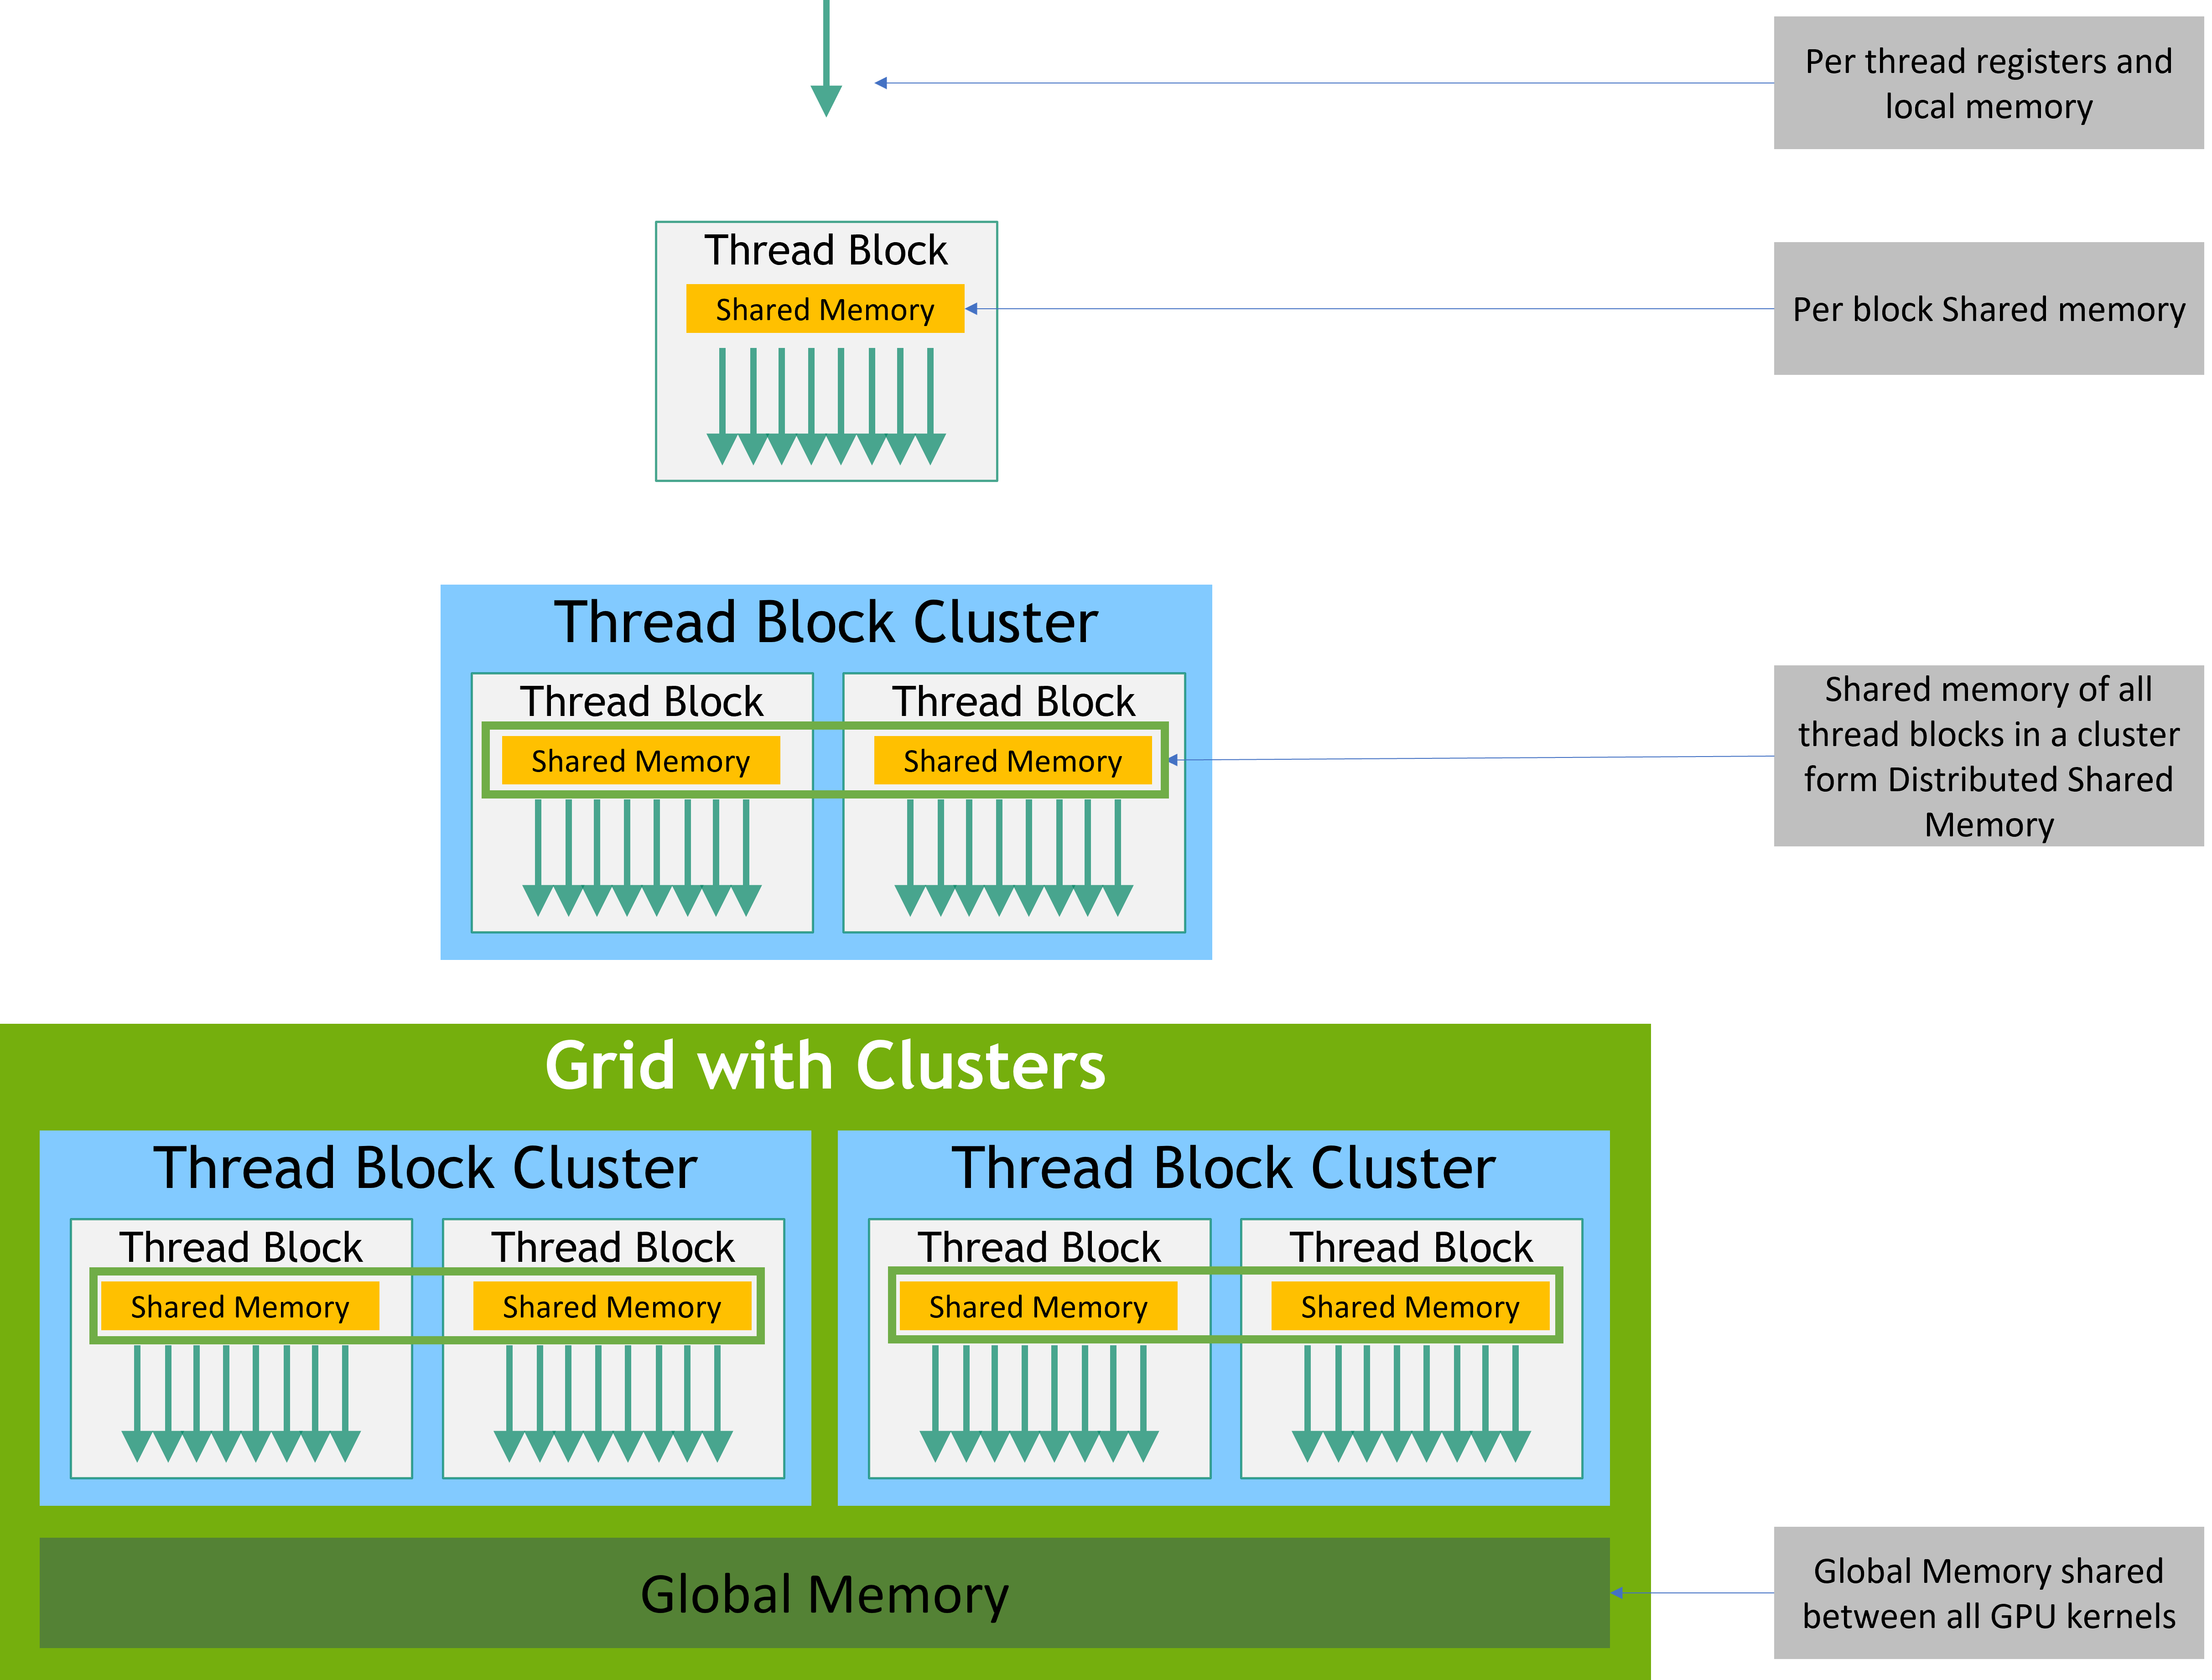
\includegraphics[scale=0.4]{src/images/memory-hierarchy.png}
    \caption{Иерархия памяти CUDA}
    \label{fig:memory_hierarchy}
\end{figure}

Программная-аппаратная модель CUDA позволяет запускать программу, написанную на языке CUDA C++, на графическом процессоре.
CUDA C++ является расширением языка C++, который позволяет объявлять C++ функции, называемые CUDA kernel,
которые будут запущены и исполнены N разными CUDA thread (далее CUDA поток). CUDA поток - это элементарная единица исполнения программы на
графическом процессоре. Ограниченный набор потоков (на данный момент, обычно до 1024) группируются в блоки (threadblock).
Каждый блок не зависит от других блоков и порядок исполнения блоков определяется аппаратной частью графического процессора, при этом каждый блок
исполняется на одном Streaming Multiprocessor (SM). Streaming Multiprocessor - это часть графического процессора, которая является
аналогом ядра в многоядерном центральном процессоре.
Блоки группируются в сетку (grid), при этом количество блоков в сетке ограничивается только диапазоном 32-битного индекса. Блок и сетка могут
иметь многомерную структура, например блок может содержать (x, y) потоков.

Важной частью программно-аппаратной модели является иерархия памяти (см. рис. \ref{fig:memory_hierarchy}). Каждый поток имеет свой собственный
набор регистров. Регистр является наиболее быстрой памятью, доступной графическому процессору. Обычно регистровый файл достаточно большой и может
содержать 255 регистров на один поток. Потоки в пределах одного блока имеют в своем распоряжении общую память (shared), которая достаточно
эффективная и является фактически программно-видимым кэшем. Обычно размеры общей памяти до 64 КБайт. Помимо этого каждый поток в каждом блоке имеет
доступ к участку оперативной памяти графического процессора, которая называется глобальная память (global). Глобальная память может достигать
размеров нескольких десятков ГБайт.

\subsection{Фреймворк машинного обучения PyTorch}
PyTorch является одним из самых часто используемых фреймворков машинного обучения \cite{pytorch_2025}\cite{pytorch_review_2024}. Это проект с открытым исходным кодом,
написанный на Python и C++, который применяется для разработки и обучения нейронных сетей. PyTorch поддерживает различные архитектуры,
в том числе центральные процессоры, графические процессоры, поддерживающие CUDA и мобильные устройства.
PyTorch содержит большое количество алгоритмов, которые используются в машинном обучении. Самые основные и важные алгоритмы являются:
\begin{itemize}
    \item операции матричного умножения
    \item операции свертки
    \item векторные/тензорные операции (сложение, скалярное произведение и т.д.)
\end{itemize}
Помимо этого, PyTorch предоставляет готовые архитектуры нейронных сетей для решения различных задач машинного обучения, например,
распознавание изображений, классификация текста и т.д.

Хоть PyTorch содержит реализации многих алгоритмов машинного обучения, Pytorch гораздо чаще использует реализации из
сторонних библиотек. Например, операции матричного умножения могут быть реализованы в библиотеке
cuBLAS \cite{cublas_2025}, операции свертки - в библиотеке cuDNN \cite{cudnn_2025} и т.д.
% В ходе исследования (см. раздел 2) было получено, что для большого числа задач PyTorch использует две библиотеки: cuBLASLt и cuDNN.
% Реализации этих библиотек является основной задачей исследования.

\subsection{CUTLASS}
Среди библиотек с открытым исходным кодом, которые могут быть использованы для реализации высокопроизводительных алгоритмов матричного умножения
и свертки особого внимания заслуживает библиотека CUTLASS \cite{cutlass_2025}.
Библиотека CUTLASS (CUDA Template Linear Algebra Subroutines) – это высокопроизводительная коллекция шаблонов и компонентов
для линейной алгебры на CUDA, разработанная NVIDIA. Она предоставляет оптимизированные реализации матричных операций
(GEMM – General Matrix Multiplication), сверток и других вычислений, используемых в глубоком обучении и
высокопроизводительных вычислениях (HPC). CU\-TLASS позволяет разработчикам создавать эффективные CUDA kernel,
используя готовые модули, что упрощает оптимизацию вычислений для различных аппаратных возможностей (например, тензорных ядер).

На момент написания данной работы библиотека CUTLASS версиии 4.0.0. Библиотека CUTLASS имеет фундаментально разные решения задач матричного
умножения и свертки в зависимости от версии. Наиболее значимые изменения свазяны с версиями 2.x и 3.x. Ввиду этого в данном обзоре будут рассматриваться
только версии CUTLASS 2.x и 3.x. Заметим, что CUTLASS является обратно совместимой с предыдущими версиями, поэтому несмотря на то, что версии 2.x и 3.x
являются более старыми, ключевые принципы организации библиотеки остаются прежними.

\subsubsection{Организация матричного умножения}
CUTLASS использует механизм шаблонов C++ для создания универсальных функций, которые могут быть использованы для реализации различных алгоритмов.
На рис. \ref{fig:cutlass_gemm} представлены основные компоненты матричного умножения для CUTLASS 2.x. Организация матричного умножения является иерархической,
что верно для большинства интерфейсов в CUTLASS. Каждый уровень организации обычно представлен каким-то шаблоном и реализует задачу своего уровня. Например,
самый нижний уровень, который называется уровнем инструкции (instruction-level) реализует примитивную операция умножения со сложение (matrix-multiply-add).
Иерархическая организация вычислений в CUTLASS соответствует модели параллелизма архитектуры CUDA и включает следующие основные уровни:
\begin{itemize}
    \item Уровень инструкции (instruction-level) — реализует примитивные операции с учетом аппаратных возможностей (например, операции умножения со сложением multiple-add)
    \item Уровень потока (thread-level) — реализует операции в рамках потока, например, работу с регистровым файлом
    \item Уровень варпа (warp-level) — реализует операции в рамках группы потоков, например, обход (iteration) матриц
    \item Уровень блока (block-level) — реализует операции в рамках блока, например, работу с глобальной памятью и общей памятью
\end{itemize}

Уровни выше, не упомянутые в списке, выполняют достаточно тривиальные операции по запуску CUDA kernel, например, выбор размер блока и
общей памяти. Стоит отметить, что эти уровни не предполагают никаких эвристик по подбору оптимальных параметров, и полностью зависят от
выбора программиста.

Так, каждый уровень выполняет какую-то конкретную задачу, например уровень блока грузит данные из
глобальной памяти в общую память соотвествующего размера, приэтом вышестоящий уровни вызывают операции уровней ниже.
Так как большинство уровней используют шаблоны, то они могут быть использованы для реализации различных алгоритмов на каждом уровне
иерархии.

\begin{figure}
    \centering
    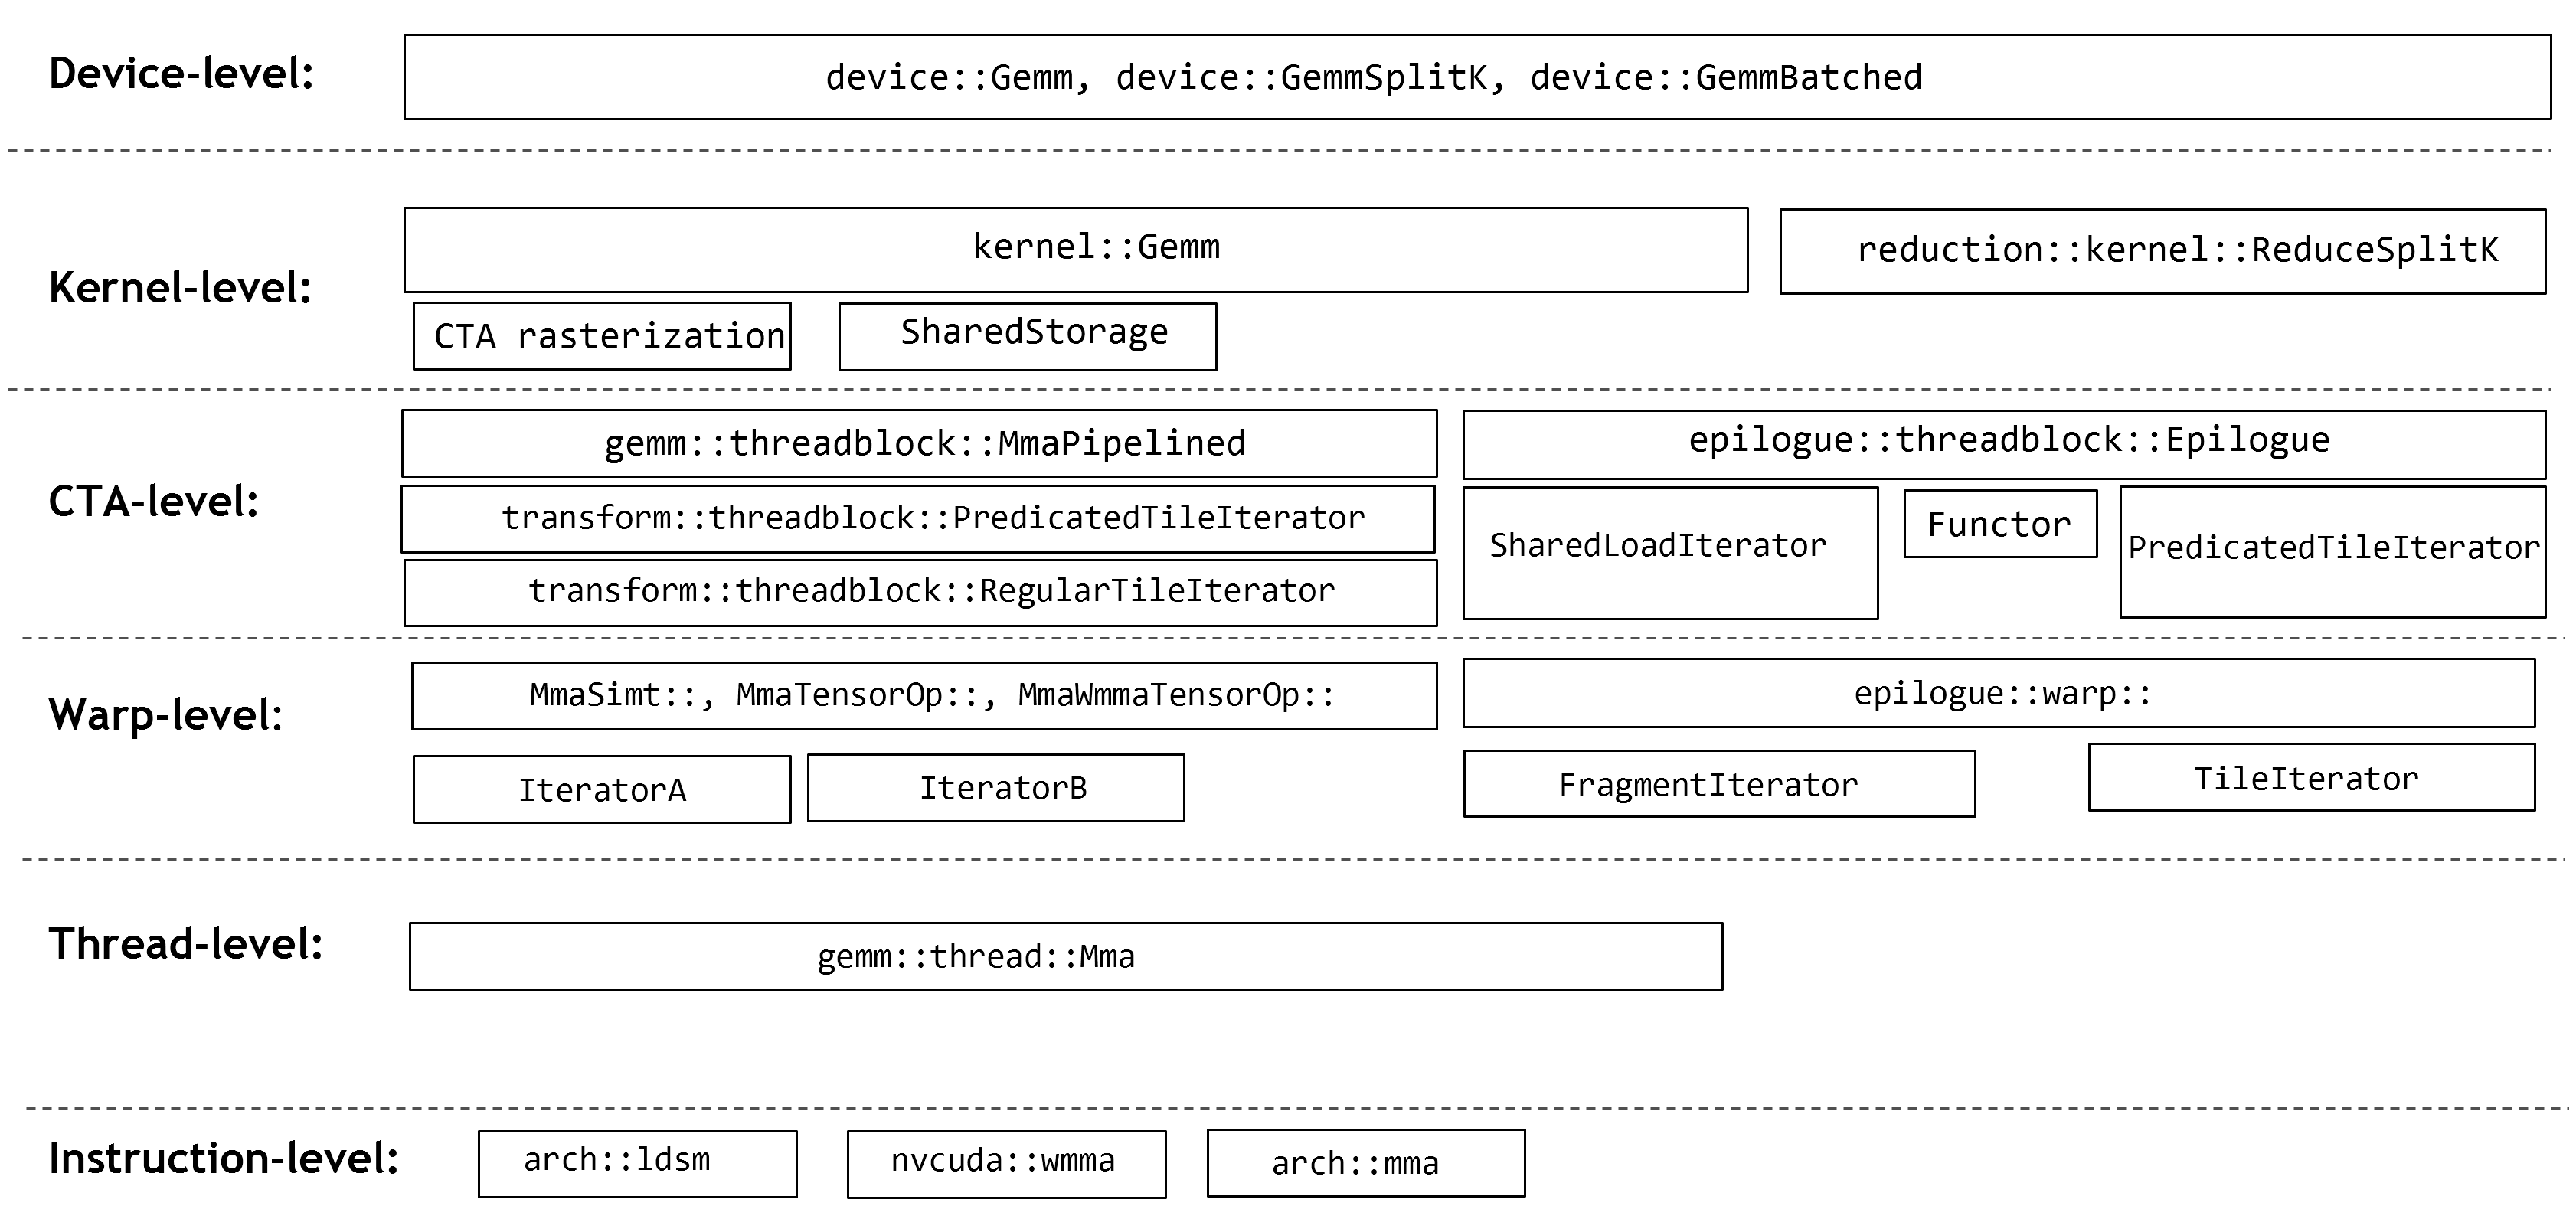
\includegraphics[scale=0.45]{src/images/cutlass-gemm-components.png}
    \caption{Основные компоненты матричного умножения для CUTLASS 2.x}
    \label{fig:cutlass_gemm}
\end{figure}


В CUTLASS 3.x основные компоненты матричного умножения представлены на рис. \ref{fig:cutlass_gemm_3.x}. В отличии от версии 2.x, где организация
полагалась на иерархию параллелизма CUDA, CUTLASS 3.x вместо этого реализует алгоритмы которые являются более универсальными и предоставляет следующие
уровни организации:
\begin{itemize}
    \item Атомарный уровень (atom-level) — реализует примитивные операции копирования (например, 64-битного числа)
    \item Уровень под-тензора (tile-level) — реализует операции в рамках под-тензора, например, копирование и умножение под-тензоров
    \item Коллективный уровень (collective-level) — является коллекцией примитов с более низких уровней, которая реализует непосредственно алгоритм матричного умножения
\end{itemize}
Самые верхние уровни, как и раньше, настраивают размеры блоков, размеры общей памяти и т.д. Такая организация позволяет сосредотачивать усилия
на реализации конкретных алгоритмов, полагаясь на оптимизированные реализации предоставляемые CUTLASS. Ключевую роль в этой организации играет
библиотека CUTE, которая позволяет описывать алгоритмы на основе примитивных операций, например, копирования, требуя меньше усилий по ансамблированию
потоков CUDA.

\begin{figure}
    \centering
    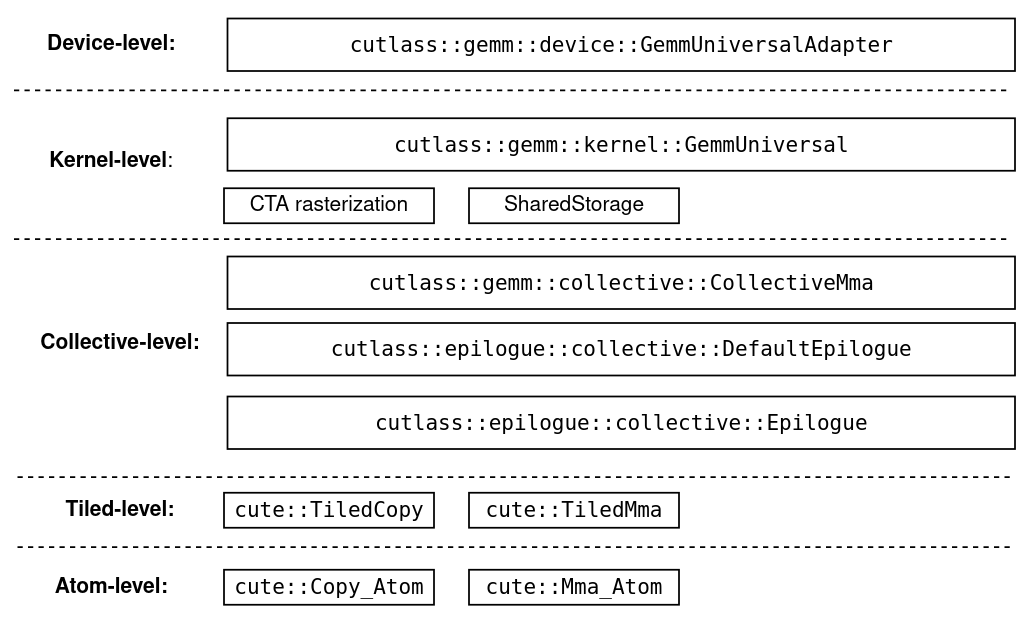
\includegraphics[scale=0.5]{src/images/cutlass-gemm3-components.png}
    \caption{Основные компоненты матричного умножения для CUTLASS 3.x}
    \label{fig:cutlass_gemm_3.x}
\end{figure}

\subsubsection{Библиотека CUTE}
В архитектуре CUTLASS 3.x ключевую роль играет библиотека CUTE, предоставляющая абстракции для реализации высокоэффективных
вычислительных алгоритмов. Данная библиотека позволяет абстрагироваться от сложностей параллельной модели выполнения CUDA.
Ключевой компонентой библиотеки CUTE является \textit{способ хранения} (далее layout), который представляет собой математические отображение:
$f \colon \mathbb{N}^n \to \mathbb{N}, где n \geq 1$, преобразующая n-мерные логические координаты в линейный индекс памяти.
Layout имеет понятие размера, то есть числа элементов, которые могут быть отображены.  Так для матрицы $A \in \mathbb{R}^{I \times J}$,
где I -- число строк, J -- число столбцов, линейный индекс в памяти вычисляется как $i \times J + j$, и является
отображением $f \colon \mathbb{N}^2 \to \mathbb{N}$, причем размером layout является $I \times J$.
Хотя логические координаты матрицы A являются двумерными (номер строки и номер столбца), CUTE позволяет использовать одномерную координату,
пересчитывая эту координату в двумерную используя колексографический порядок ("справа-налево").
Например, в случае матрицы A схема перевода будет следующая: 0 $\mapsto$ (0, 0), 1 $\mapsto$ (1, 0), 2 $\mapsto$ (2, 0), ... I $\mapsto$ (I, 0),
I + 1 $\mapsto$ (0, 1), I + 2 $\mapsto$ (1, 1), ... I $\times$ J $\mapsto$ (I, J).

Для layout реализованы операции \textit{слияния} (coalescing), \textit{композиции} (composition) и \textit{дополнения} (complement).
Операция слияния упрощает пересчет логических координат в линейный индекс, посредством упрощения формулы перевода координат.
Например, для вырожденного трехмерного массива $T \in \mathbb{R}^{K \times 1 \times M}$, операция слияния уменьшает размерность задачи,
сохряняя правильное отображение. Библиотека CUTE имеет множество статических проверок свойств отображений и позволяет упрощать вычисления
свазянные с layout, что имеет решающую роль в виду высокой цены вычислений такого рода операций на GPGPU.

Операция композиции позволяет объединить два отображения $f_1 \colon \mathbb{N}^n \to \mathbb{N}$ и $f_2 \colon \mathbb{N}^k \to \mathbb{N}$
в одно отображение $f_1 \circ f_2 \colon \mathbb{N}^m \to \mathbb{N}$, такое, что $f_1 \circ f_2(x) =$ $f_1$($f_2$(x)), где x -- логические
координаты отображения $f_2$ (не более чем k-мерный вектор). Такая композиция возможна, потому что как уже отмечалось выше, в CUTE можно вместо логических
координат использовать координаты меньше размерности, пересчитывая их в логические используя колексографический порядок. Композиция крайне полезная
операция, которая используется для того, чтобы делить массивы на подмассивы. Действительно, по определению композиции мы используем логических координаты
отображения $f_2$, которая затем переводится в логические координаты отображения $f_1$. Однако, не сложно понять, что при операции композиции мы можем
перебрать не все логические координаты $f_1$, что означает что мы обращаемся не по каждому линейному индексу в памяти. Для этого была введена операция
дополнения.

Операция дополнения можно описать как отображение $f^*$, такое что $f^*(i) \neq f(j)$, причем $0 \leq i \leq I$, и $0 \leq j \leq J$, а I + J = K, где
K какое-то конечное натуральное число. Такого рода операция полезна, когда мы обращаемся к подмассиву в каком-то массив, используя операцию композиции,
но приэтом не обращаемся ко всем элементам этого массива. Тогда дополнение будет такой layout, который будет обращаться только к тем элементам,
которые не доступны через композицию. Таким образом, через введенные три операции решается сложная задача по делению массива на подмассивы,
которая имеет решающее значение в виду высокой параллельности GPGPU и необходимости распределения вычислений по потокам.

\subsubsection{Организация свертки}
Свертка является операцией над многомерными массивами (чаще называемые тензорами). Рассмотрим наиболее распостранненый случай 4-мерных тензоров:
\begin{equation}
\label{eq:conv}
y[n,p,q,k] = \sum_{c=0}^{C-1} \sum_{r=0}^{R-1} \sum_{s=0}^{S-1} x[n, \tilde{h}(p,r), \tilde{w}(q,s), c] \cdot w[k,c,r,s]
\end{equation},
где:
\begin{itemize}
    \item $\mathbf{x} \in \mathbb{R}^{N \times H \times W \times C}$ -- входной тензор (батч изображений)
    \item $\mathbf{w} \in \mathbb{R}^{K \times C \times R \times S}$ -- тензор фильтров
    \item $\mathbf{y} \in \mathbb{R}^{N \times P \times Q \times K}$ -- выходной тензор
\end{itemize}

Координаты $\tilde{h}$ и $\tilde{w}$ определяются следующим образом:
\begin{align}
\tilde{h}(p,r) &= p \cdot s_h - p_h + r \cdot d_h \label{eq:coord_transform_h} \\
\tilde{w}(q,s) &= q \cdot s_w - p_w + s \cdot d_w \label{eq:coord_transform_w}
\end{align}

Параметры свертки:
\begin{itemize}
    \item $s_h, s_w$ -- шаг свертки (stride)
    \item $p_h, p_w$ -- дополнение (padding)
    \item $d_h, d_w$ -- коэффициент расширения (dilation)
\end{itemize}

Представленная формула \eqref{eq:conv} описывает наиболее распространённый случай двумерной свертки для четырёхмерных тензоров.
Однако, операция свертки может быть обобщена на тензоры произвольной размерности.

Операция свертки, также как и матричного умножения имеет иерархическую структуру. В библиотеке CUTLASS методом расчета свертки является
сведение его к матричному умножению (метод \textit{implicit GEMM convolution}), поэтому иерархия операций свертки аналогично иерархии операций
матричного умножения, с поправкой на то, что классы реализующие операцию свертки имеют другое имя (см. рис. \ref{fig:cutlass_gemm} и рис.
\ref{fig:cutlass_gemm_3.x}). Данный метод расчета используется преимущественно для четырёхмерных тензоров. Для данных тензоров есть два наиболее
распостряненных формата: NCHW и NHWC. Здесь N -- количество изображений, C -- количество каналов, H -- высота изображения, W -- ширина изображения.
Форматы NCHW и NHWC являются способами хранения многомерного массива в линейной памяти, приэтом названия форматов описывают порядок координат.
На данный момент, расчет свертки в CUTLASS через матричного умножения реализован только для формата NHWC. Идея расчета заключается в сведении 4-мерных
тензоров в 2-мерные матрицы А, B C по следующей схеме: $\mathbf{x}$[N, H, W, C] $\mapsto$ A[NPQ, RSC], $\mathbf{w}$[K, C, R, S] $\mapsto$ B[RSC, K],
$\mathbf{y}$[N, P, Q, K] $\mapsto$ C[NPQ, K] (см. рис. \ref{fig:implicit_gemm_algo}). Таким образом, свертка сводится к задаче матричного умножения
вида:
\begin{equation}
\mathbf{C}[\tilde{m}, \tilde{n}] = \mathbf{A}[\tilde{m}, \tilde{k}] \cdot \mathbf{B}[\tilde{k}, \tilde{n}],
\end{equation},
где:
\begin{align}
&0 \leq \tilde{m} \leq \tilde{M} = N \cdot P \cdot Q, \\
&0 \leq \tilde{n} \leq \tilde{N} = K, \\
&0 \leq \tilde{k} \leq \tilde{K} = R \cdot S \cdot C.
\end{align}

\begin{figure}
    \centering
    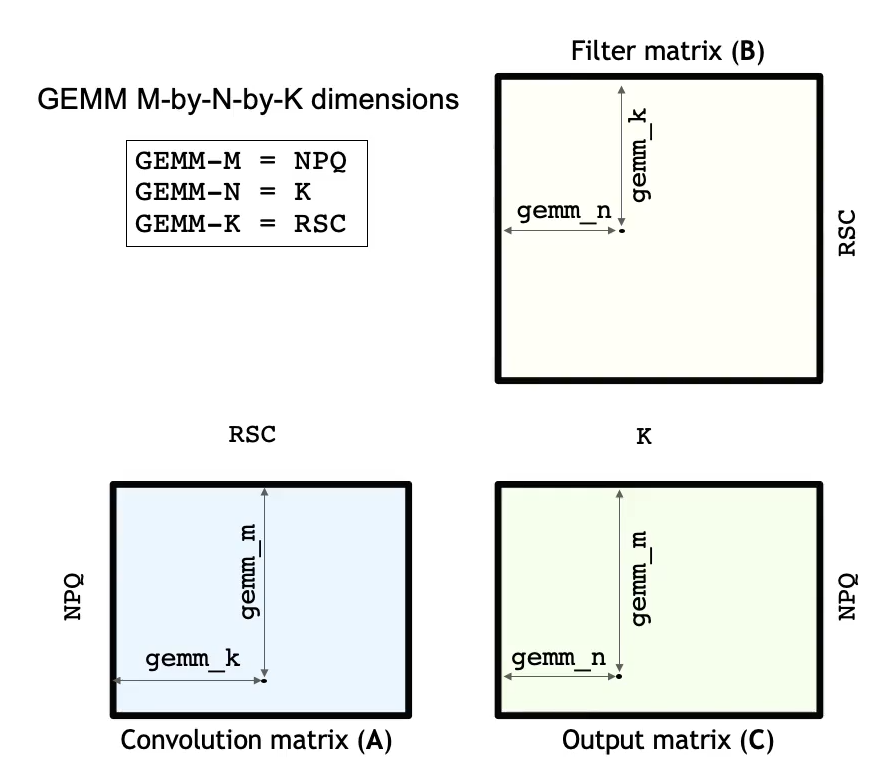
\includegraphics[scale=0.5]{src/images/implicit_gemm_algo.png}
    \caption{Сведение операции свертки к матричному умножению}
    \label{fig:implicit_gemm_algo}
\end{figure}

Важно, что такое сведение не предполагает выделение допольнительной памяти, а только пересчет координат из 4-мерного тензора в 2-мерную матрицу.
Таким образом, можно использовать эффективные алгоритмы матричного умножения для ускорения расчета свертки, но приэтом нужно тратить вычислительные
ресурсы на пересчет координат. Для решения этой задачи CUTLASS переиспользует большую часть кода для матричного умножения.
Структурно CUTLASS 2.x меняет только схему загрузки данных из глобальной памяти в общую память, остальная же часть остается прежней
(см. рис. \ref{fig:implicit_gemm_struct} -- здесь зеленым цветом обозначены измененные части по сравнению с матричным умножением).
\begin{figure}
    \centering
    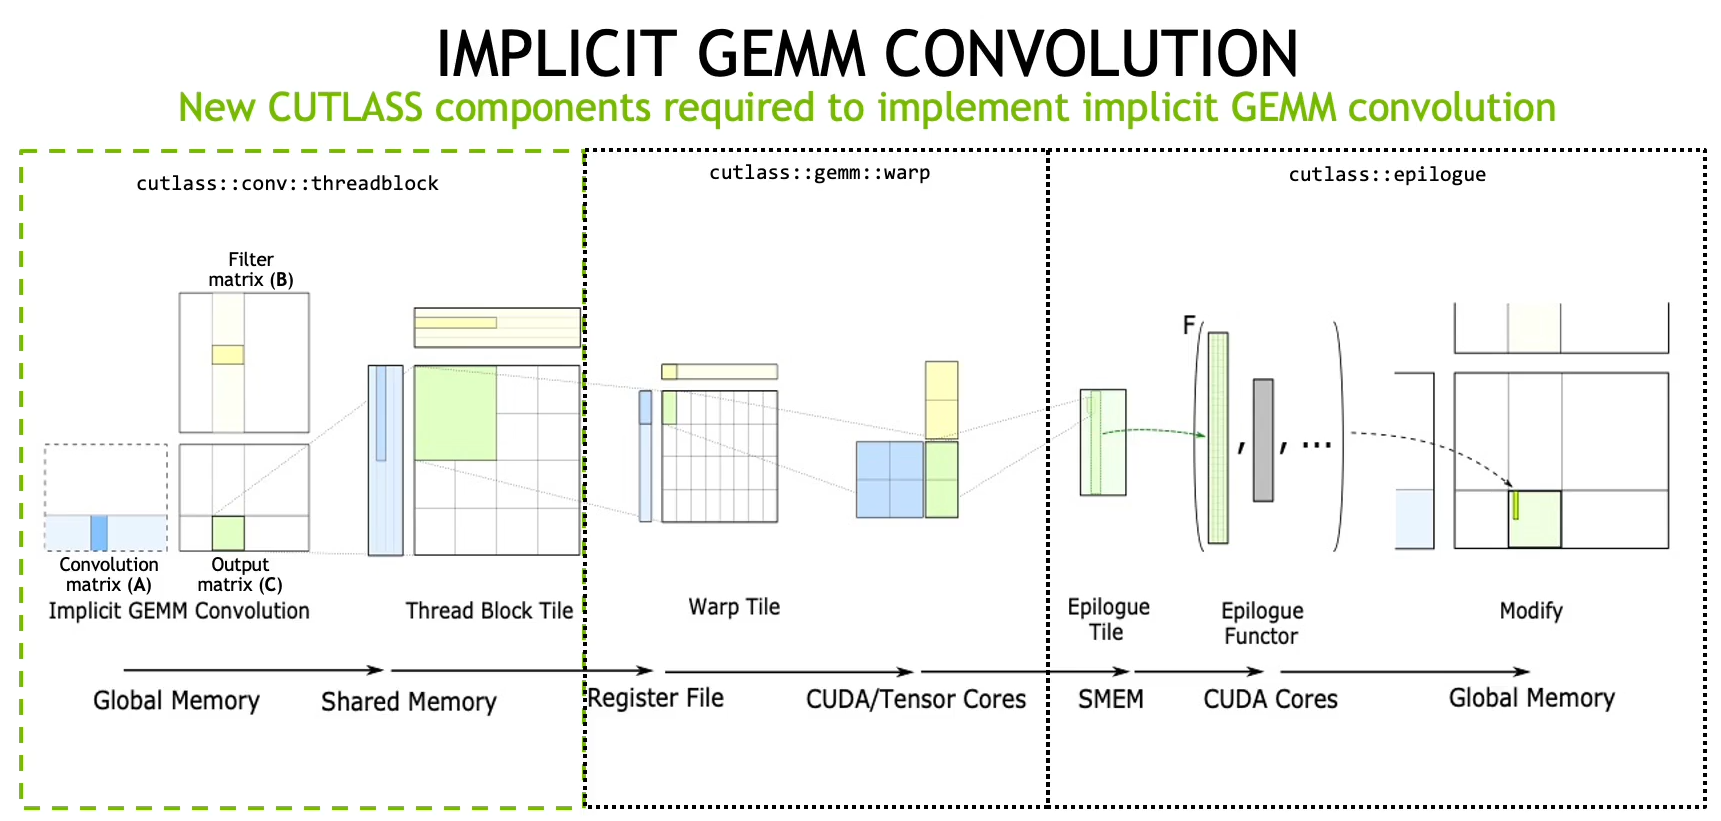
\includegraphics[scale=0.35]{src/images/implicit_gemm_struct.png}
    \caption{Структура метода расчета свертки через матричное умножение}
    \label{fig:implicit_gemm_struct}
\end{figure}

\subsubsection{Сравнение с библиотеками cuBLAS и cuDNN}
\label{subsec:comparison}

Библиотека CUTLASS демонстрирует высокую производительность при решении задач линейной алгебры и машинного обучения, однако обладает рядом
ограничений по сравнению с cuBLAS и cuDNN. Наиболее существенными являются:
\begin{enumerate}
\item \textbf{Автоматизация выбора алгоритмов}:
\begin{itemize}
\item В CUTLASS разработчик должен вручную выбирать и настраивать параметры алгоритмов
\item Библиотеки cuBLAS и cuDNN предоставляют автоматический выбор оптимальных реализаций на основе:
\begin{itemize}
\item Параметров задачи (размерности матриц/тензоров)
\item Аппаратных характеристик GPU
\item Требуемой численной точности
\end{itemize}
\end{itemize}

\item \textbf{Степень поддержки операций машинного обучения}:
    \begin{itemize}
    \item Отсутствие поддержки NCHW для совместимости с PyTorch
    \item Отсутствие реализации пакетной нормализации
    \end{itemize}
\end{enumerate}

Особую важность представляет поддержка формата NCHW, который является стандартом де-факто в большинстве фреймворков машинного обучения, включая PyTorch.
Отсутствие этой функциональности существенно ограничивает применимость CUTLASS в промышленных решениях.

Менее критичным ограничением является более низкие показатели производительности. В разделе \ref{sec:survey} показано, что CUTLASS в задачах матричного умножения
достигает 90-95\% производительности cuBLAS. Для создания полноценной аналогов cuBLAS и cuDNN необходимо разработать систему автоматического выбора алгоритмов,
расширить поддержку операций машинного обучения и провести оптимизацию алгоритмов.
	\clearpage

	
\section{Обзор существующих решений}
TBD; \textit{Чуть более подробно}
\subsection{cuBLAS}
cuBLAS (CUDA Basic Linear Algebra Subprograms) - это высокооптимизированная библиотека линейной алгебры,
разработанная NVIDIA для своих графических процессоров. Она предоставляет реализации стандартных операций линейной алгебры такие как:
\begin{itemize}
    \item векторные операции (сложение, скалярное произведение)
    \item умножение матрицы на вектор
    \item умножение матрицы на матрицы
\end{itemize}
cuBLAS включает в себе разные подбиблиотеки, например, cuBLASLt. cuBLASLt - это облегченная версия библиотеки, представленная в
CUDA 10.1, которая предлагает более гибкий API и специализированные функции для матричных умножений.
Ключевым преимуществом cuBLAS является автоматический выбор оптимального алгоритма для конкретной операции с учетом того, на каком
устройстве будет выполняться вычисление.
Проблема библиотеки cuBLAS в том, что она является библиотекой с закрытым исходным кодом, что делает невозможным перекомпиляцию
их для запуска на функциональном и потактовом симуляторе графического процессора. Помимо этого исходный код cuBLAS представляет
большой интерес для исследования нюансов работы графического процессора и его устройства.

\subsection{cuDNN}
cuDNN (CUDA Deep Neural Network library) — это высокопроизводительная библиотека от NVIDIA, предоставляющая оптимизированные реализации примитивов
для глубокого обучения. Разработанная специально для ускорения нейронных сетей на GPU, она стала стандартом в индустрии и используется всеми
основными фреймворками машинного обучения, в том числе PyTorch.
Она предоставляет оптимизированные реализации следующих операций:
\begin{itemize}
    \item сверточные операции:
    \begin{itemize}
        \item Прямая/обратная свертка
        \item Поддержка различных форматов тензоров (NCHW, NHWC, и т.д.)
    \end{itemize}
    \item Пуллинг операции
    \item Нормализация
    \item Функции активации
\end{itemize}

Также как и cuBLASLt, cuDNN автоматически подбирает оптимальную реализацию для каждой конкретной операции.
Аналогично, cuDNN проект с закрытым исходным кодом.


	\clearpage

	
\section{Исследование и описание решения задачи}
\label{sec:survey}
\subsection{Стратегия разработки}
\label{subsec:develop_strat}

\begin{table}[h]
\centering
\begin{tabular}{|c|c|c|}
\hline
\begin{tabular}[c]{@{}c@{}}Название \\ нейронной\\ сети\end{tabular} & Ссылка на статью         \\ \hline
\textbf{Задача классификации:}                                       &                          \\ \hline
Resnet                                                               & \cite{resnet_2015}       \\ \hline
EfficientNet                                                         & \cite{efficientnet_2019} \\ \hline
Resnext                                                              & \cite{resnext_2016}      \\ \hline
SimpleViT                                                            & \cite{simplevit_2022}    \\ \hline
Swin Transformer V2                                                  & \cite{swin_2021}         \\ \hline
DINOv2                                                               & \cite{dinov2_2024}       \\ \hline
CLIP                                                                 & \cite{clip_2021}         \\ \hline
MoViNet                                                              & \cite{movinet_2021}      \\ \hline
\textbf{Задача детекции:}                                            &                          \\ \hline
YOLOv11                                                              & \cite{yolov11_2024}      \\ \hline
\textbf{Задача сегментации:}                                         &                          \\ \hline
UNET/UNET+/UNET++                                                    & \cite{unet_2015}         \\ \hline
SAM/SAM2                                                             & \cite{sam2_2024}         \\ \hline
\end{tabular}
\caption{Список моделей для тестирования}
\label{tbl:models}
\end{table}

Разработка полнофункциональных аналогов библиотек cuBLAS и cuDNN представляет собой
обширную инженерную задачу, требующую четкого определения приоритетов. Выбор фокуса разработка сильно обусловлен
спецификой целевой платформы. Например, на встраиваемых системах Nvidia Jetson задачи вывода (inference) составляют основной
рабочий сценарий. Разрабатываемый GPGPU ускоритель предполагает схожие сценарии работы, поэтому основным приоритетом является
inference-режим.

Учитывая, что библиотеки cuBLAS и cuDNN преимущественно используются через высокоуровневые фреймворки (PyTorch, TensorFlow),
критически важными становятся бесшовная интеграция с существующими API, соответствие ожидаемому поведению в реальных сценариях
и стабильность работы в составе сложных задач машинного обучения. В качестве референсной платформы для верификации предлагается
использовать PyTorch, что обеспечивает:
\begin{itemize}
\item Доступ к широкому спектру готовых моделей (ResNet, BERT, YOLO)
\item Тестовое покрытие на реальных задачах
\item Возможность интеграции с инструментами профилирования Nvidia Nsight \cite{nsight_systems_2025}
\end{itemize}
Для систематизации процесса разработки аналогов библиотек cuBLAS и cuDNN был проведен анализ функций,
наиболее востребованных при работе с нейронными сетями в режиме вывода (inference).
Принято решение о фиксации набора эталонных моделей, которые удовлетворяют следующим критериям отбора:
\begin{itemize}
    \item Широкая распространенность в промышленных решениях
    \item Соответствие требованием заказчика GPGPU ускорителя
\end{itemize}

Отобранные модели работали в режиме вывода и представлены в табл. \ref{tbl:models}. После фиксации моделей
были зафиксированы все интерфейсы библиотек cuBLAS и cuDNN c помощью утилиты трассирования \textit{ltrace}.
Анализ показал, что во всех представленных сетях больше всего задействованы следующие вызовы:
\begin{itemize}
   \item \textbf{cuBLAS}
    \begin{itemize}
        \item \texttt{cublasLtMatmul} — общее матричное умножение (GEMM — general matrix multiplication)
    \end{itemize}

    \item \textbf{cuDNN}
    \begin{itemize}
        \item \texttt{cudnnConvolutionForward} — прямая свертка тензора (обычно 4-мерного в формате NCHW или NHWC)
        \item \texttt{cudnnBatchNormalizationForwardInference} — пакетная нормализация тензора
    \end{itemize}
\end{itemize}

\subsection{Схема запуска на симуляторе gem5}

\begin{figure}
    \centering
    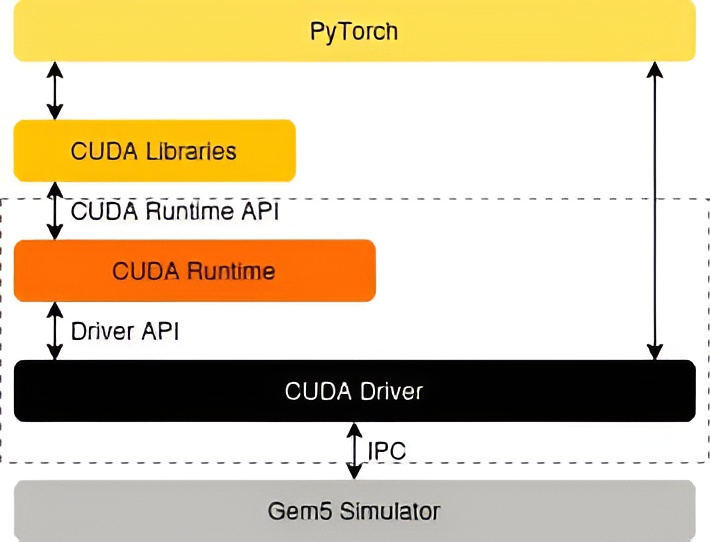
\includegraphics[scale=0.4]{src/images/launch_scheme.jpeg}
    \caption{Запуск приложения на функциональном/потактовом симуляторе}
    \label{fig:launch_scheme}
\end{figure}

Представленные нейронные сети должны быть запущены на функциональном и потактовом симуляторе GPGPU, поддерживающего модель CUDA.
На рисунке \ref{fig:launch_scheme} представлена архитектурная схема выполнения нейронных сетей из таблицы \ref{tbl:models}
на функциональном и потактовом симуляторе. Как следует из схемы, процесс выполнения в PyTorch включает
многоуровневую систему вызовов.

При запуске нейронной сети фреймворк PyTorch обращается к функциям библиотек cuBLAS и cuDNN, которые содержат реализации вычислительных
алгоритмов в виде CUDA kernel. При запуске CUDA kernel вызываются функции библиотеки времени выполнения (например, \texttt{cudaLaunchKernel})
и функции драйвера устройства.

Библиотека времени выполнения предоставляет высокоуровневый API для управления вычислительным устройством.
Драйвер устройства обеспечивает непосредственное взаимодействие с аппаратными ресурсами
через набор низкоуровневых интерфейсов. Библиотека времени выполнения использует низкоуровневые интерфейсы драйвера
для реализации своего функционала.

В предложенной архитектуре драйвер устройства через механизм межпроцессорного взаимодействия (IPC) передает вычислительные задачи на
симулятор, который эмулирует выполнение соответствующих CUDA kernel. Для преобразования исходного кода CUDA в исполняемый формат
используется специализированный компилятор на базе инфраструктуры LLVM \cite{llvm_project_2025}, обеспечивающий оптимизацию под целевую платформу.

\subsection{Методология тестирования}
При разработке GPGPU критически важным является верификация результатов вычислений. При этом разработка значительно упрощается
при наличии эталонной реализации. В качестве эталонной платформы выбраны устройства компании Nvidia, что обусловлен их доминирующим
положение на рынке ускорителей для машинного обучения.

При тестировании \textit{функциональной} корректности библиотек cuBLAS и cuDNN архитектурные особенности реализации (такие как конвейерная
обработка команд или организация иерархии памяти) не являются определяющими факторами. Это позволяет существенно оптимизировать процесс
тестирования, разделив его на два параллельных направления. Основной объем тестирования выполняется на реальных устройствах NVIDIA Jetson,
что имеет следующие ключевых преимущества:
\begin{itemize}
    \item Высокая скорость выполнения тестовых прогонов по сравнению с симулятором
    \item Возможность быстрых итераций при разработке
    \item Проверка библиотек в реальных условиях
\end{itemize}
Параллельно осуществляется тестирование на симуляторе, которое фокусируется на осуществлении соответствия
семантики исполнения инструкции, описанными в документе разрабатываемого ускорителя.

Как уже отмечалось были зафиксированы три ключевых интерфейса: \texttt{cublasLtMatmul}, \texttt{cudnnConvolutionForward},
\texttt{cudnnBatchNormalizationForwardInference}, которые используются нейронными сетями из табл. \ref{tbl:models}. Помимо этого
были сняты все параметры интерфейсов, включая:
\begin{itemize}
    \item Размерности тензоров
    \item Тип данных и формат хранения
    \item Параметры операции, такие как шаг свертки
    \item Дополнительные параметры, регулирующие выбор алгоритмов
\end{itemize}
Далее были построены тесты, которые сравнивали эталонную реализацию cuDNN и cuBLAS с разрабатываемыми аналогами в описанных сценариях
с необходимой точностью.

\subsection{Методология оценки производительности}
\label{subsec:perf_eval}
В отличие от функционального тестирования, анализ производительности требует более детального и системного подхода.
Разработка конкурентоспособного GPGPU-ускорителя предполагает достижение высокой эффективности при выполнении промышленных
задач, что обуславливает необходимость комплексной методики измерений.

Основным инструментом для точной оценки временных характеристик разрабатываемой архитектуры служит тактовый (cycle-accurate) симулятор
на базе платформы gem5. Данный инструментарий позволяет получить детальную информацию о ключевых метриках производительности, такие как
количество тактов, статистика работы иерархии памяти, загрузку вычислительных блоков.

Однако необходимо отметить, что потактовые симуляторы характеризуются чрезвычайно высокой вычислительной стоимостью,
что существенно ограничивает их применение для оперативной оценки производительности в процессе разработки.

Учитывая архитектурную близость разрабатываемого решения к GPU NVIDIA, была принята методика кросс-валидации
производительности на реальных устройствах серии Jetson Xavier. Данный подход основан на следующих допущениях:
\begin{itemize}
    \item Оптимизированные для архитектуры NVIDIA задачи демонстрируют сопоставимую эффективность на разрабатываемом ускорителе
    \item Относительные показатели производительности сохраняются
    \item Принцип написания высокоэффективного CUDA-кода коррелируют между платформами
\end{itemize}

Таким образом, в данной работе большее внимание уделена анализу производительности и функциональной корректности
на реальных графических процессора Nvidia.

\subsection{Реализация операция \texttt{cublasLtMatmul}}
% \subsubsection{Описание возможностей}
Операция \texttt{cublasLtMatmul} реализует обобщенное матричное умножение с возможностью дополнительных преобразований.
Формально операция определяется следующим образом:

Пусть заданы:
\begin{itemize}
    \item $\mathbf{A} \in \mathbb{F}^{M \times K}$ - входная матрица
    \item $\mathbf{B} \in \mathbb{F}^{K \times N}$ - входная матрица
    \item $\mathbf{C} \in \mathbb{F}^{M \times N}$ - дополнительная матрица
    \item $\mathbf{D} \in \mathbb{F}^{M \times N}$ - результирующая матрица
\end{itemize}

Тогда результат вычисляется по формуле:
\begin{equation}
\mathbf{D} = \text{epilogue}\left(\alpha \cdot \text{op}(\mathbf{A}) \cdot \text{op}(\mathbf{B}) + \beta \cdot \text{op}(\mathbf{C})\right)
\end{equation}

где:
\begin{itemize}
    \item $\text{op}(\cdot)$ - оператор преобразования матрицы (тождественный, транспонирование или эрмитово сопряжение)
    \item $\text{epilogue}(\cdot)$ - постобработка результата (например, функция активации ReLU)
    \item $\alpha, \beta \in \mathbb{F}$ - скалярные коэффициенты
    \item $\mathbb{F}$ - некоторое поле, обычно $\mathbb{R}$ или $\mathbb{C}$
\end{itemize}

Размерности матриц должны удовлетворять условию согласованности: если $\text{op}(\mathbf{A})$ имеет размер
$m \times k$, а $\text{op}(\mathbf{B})$ - размер $k \times n$, то $\text{op}(\mathbf{C})$ должен иметь размер $m \times n$.

Среди возможных функций постобработки часто применяется \textit{вектор смещений}.
В контексте матричных операций под вектором смещений (bias vector) понимается операция вида:
\begin{equation}
D_{i,j} = \left(\alpha \cdot (\mathbf{A}\mathbf{B})_{i,j} + \beta \cdot C_{i,j}\right) + b_j \quad \text{для} \quad i=1,\ldots,M; \ j=1,\ldots,N
\end{equation}

где:
\begin{itemize}
    \item $b_j$ - $j$-тый элемент вектора смещений
    \item Сложение с вектором выполняется путем его неявного расширения (broadcasting) по строкам
\end{itemize}

Помимо базовой реализации матричного умножения, операция \texttt{cublasLtMatmul} поддерживает возможность пакетной обработки
(\textit{batched GEMM}). Формально операция описывается как:
\begin{equation}
\mathbf{D}_i = \text{epilogue}\left(\alpha \cdot \text{op}(\mathbf{A}_i) \cdot \text{op}(\mathbf{B}_i) + \beta \cdot \text{op}(\mathbf{C}_i)\right), \quad i = 1,\ldots,N
\end{equation}
Опять же матрицы должны удовлетворять условию согласованности размеров.

% \subsubsection{Тестовая выборка}
\begin{table}[h]
\centering
\begin{tabular}{|l|c|c|r|}
\hline
\multicolumn{1}{|c|}{\textbf{Тип данных}} & \textbf{Батчинг} & \textbf{Эпилог} & \textbf{Кол-во тестов} \\ \hline
float32 & Нет & Вектор смещений & 29 \\ \hline
float32 & Да & Нет & 19 \\ \hline
complex32 & Да & Нет & 123 \\ \hline
complex32 & Нет & Нет & 7 \\ \hline
\hline
\multicolumn{3}{|l|}{\textbf{Всего:}} & 178 \\ \hline
\end{tabular}
\caption{Классификация вызовов \texttt{cublasLtMatmul} по типам операций}
\label{tbl:cublas_calls}
\end{table}

В таблице \ref{tbl:cublas_calls} приведены все вызовы операции \texttt{cublasLtMatmul}, которые были зафиксированы по методологии,
описанной в разделе \ref{subsec:develop_strat}. Все вызовы были систематизированы по трем ключевым параметрам:
\begin{itemize}
\item Типу обрабатываемых данных (вещественные или комплексные числа)
\item Наличию пакетной обработки (\textit{batching})
\item Применению дополнительных преобразований (эпилогу)
\end{itemize}

% \subsubsection{Параметры конфигурации GEMM в CUTLASS: влияние на загрузку потоков и производительность}
Анализ возможностей библиотеки CUTLASS показал, что CUTLASS поддерживает необходимый функционал для
реализации операции \texttt{cublasLtMatmul}. В CUTLASS имеется реализации пакетной обработки и операций
с комплексными числами, однако есть ограничения на вектор смещений. На момент написания реализации \texttt{cublasLtMatmul}
CUTLASS не поддерживал одновременное использование матрицы $\mathbf{C}$ и вектора смещений.

В отличие от библиотеки cuBLAS, которая автоматически выбирает оптимальные алгоритмы для заданных параметров задачи,
CUTLASS требует явного указания вычислительных параметров через шаблонные классы.
Для оценки производительности использовалась платформа NVIDIA Jetson Xavier, архитектурные характеристики которой наиболее
близки к разрабатываемому GPGPU-ускорителю.

Ключевым параметром, определяющим производительность на данной платформе, являются размеры подматриц, обрабатываемых отдельными
блоками и варпами. В CUTLASS 2.x эти параметры задаются шаблонным классом \texttt{cutlass::GemmShape<\~{M}, \~{N}, \~{K}>}, где для матрицы
$\mathbf{A}$ выделяется подматрица размера $\tilde{M} \times \tilde{K}$, для $\mathbf{B}$ - $\tilde{K} \times \tilde{N}$, а для результирующей
матрицы $\mathbf{D}$ - $\tilde{M} \times \tilde{N}$.

Конкретный пример с размерами подматриц для блока \texttt{cutlass::GemmShape<128, 64, 8>} определяет следующие характеристики:
\begin{itemize}
    \item Требования к общей памяти:
    \begin{itemize}
        \item Для матрицы $A$: $128 \times 8 \times \text{размер элемента}$
        \item Для матрицы $B$: $64 \times 8 \times \text{размер элемента}$
    \end{itemize}
    \item Область данных, параллельно обрабатываемую одним CUDA-блоком
\end{itemize}

\begin{figure}[h]
    \centering
    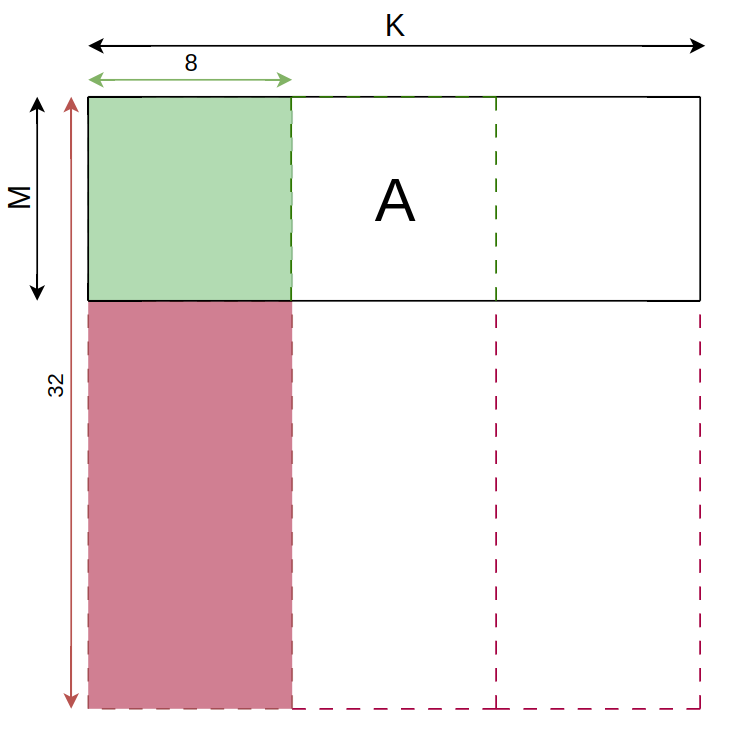
\includegraphics[width=0.8\textwidth]{src/images/block_sizes_no_grid.png}
    \caption{Пример неоптимального выбора параметров ($\tilde{M}=32$ для $M<32$): красным выделены простаивающие потоки}
    \label{fig:block_sizes}
\end{figure}

В CUTLASS для утилизирования тензорных инструкций [x] также располагает размерами подматрица, обрабатываемых отдельными потоками.
В рассматриваемой реализации каждый поток обрабатывает один элемент матрицы, что задаётся параметром \texttt{cutlass::GemmShape<1, 1, 1>}.
Такой выбор связан с тем, что в тестах отобраны вызовы не предполагающие использование тензорных инструкций.
В совокупности с размерами подматриц, обрабатываемых отдельными варпами, можно однозначно определить количество варпов в блоке и соотвественно
количество потоков в блоке.

Выбор оптимальных значений $\tilde{M}$, $\tilde{N}$ и $\tilde{K}$ может учитывать:
\begin{itemize}
    \item Размера исходных матриц
    \item Ограничения по размеру общей памяти
    \item Особенности планирования варпа на целевой архитектуре
\end{itemize}

Для определения оптимальных значений $\tilde{M}$ и $\tilde{N}$ предложен простой и эффективный метод,
основанный на анализе размеров исходных матриц. Алгоритм для $\tilde{M}$ (аналогично для $\tilde{N}$) описывается следующим образом:

Пусть:
\begin{itemize}
    \item $M$ -- размер исходной матрицы по строкам
    \item $L = \{16, 32, 64, 128\}$ -- множество допустимых размеров подматриц (степени двойки)
\end{itemize}

Тогда оптимальное значение $\tilde{M}$ определяется как:
\begin{equation}
\tilde{M} =
\begin{cases}
\max \{ l \in L \mid l \leq M \}, & \text{если } M \geq 16 \\
16, & \text{если } M < 16
\end{cases}
\end{equation}

Как показано на рис. \ref{fig:block_sizes}, выбор $\tilde{M}=32$ для матрицы с $M<32$ приводит к значительному простою потоков (выделены красным).
Предложенный алгоритм позволяет увеличить отношение работающих потоков к простаивающим и обеспечить более высокую загрузку вычислительных блоков.

\begin{figure}[ht]
\centering
\begin{tikzpicture}
\begin{axis}[
    ybar,
    width=0.5\textwidth,
    height=0.6\textwidth,
    bar width=0.5cm,
    ymajorgrids=true,
    ylabel={Производительность относительно cuBLAS},
    ymin=0,
    ymax=1,
    symbolic x coords={CUTLASS, CUTLASS+оптимизация},
    xtick=data,
    nodes near coords,
    nodes near coords align={vertical},
    every node near coord/.append style={font=\small, yshift=5pt},
    axis lines*=left,
    tick label style={font=\small},
    label style={font=\small},
    title style={font=\small, align=center},
    title={Сравнение производительности реализаций \\ интерфейса \texttt{cublasLtMatmul}},
    enlarge x limits=0.4
]

\addplot[fill=blue!30, draw=blue!80] coordinates {
    (CUTLASS, 0.35)
    (CUTLASS+оптимизация, 0.9)
};

\end{axis}
\end{tikzpicture}
\caption{Сравнение производительности разработанного решения с cuBLAS на Jetson Xavier: геометрическое среднее
относительного ускорения до и после применения оптимизации}
\label{fig:cublas_bar}
\end{figure}

Количественная оценка эффективности предложенного подхода представлена на рис. \ref{fig:cublas_bar}. Тестирование проводилось на
платформе Nvidia Jetson Xavier по методологии, описанной в разделе \ref{subsec:perf_eval} с использованием тестовых сценариев из таблицы
\ref{tbl:cublas_calls}.

Результаты показывают, что оптимизированная реализация достигает 90\% производительности эталонной библиотеки cuBLAS, что свидетельствует о высокой
эффективности предложенных решений.

\subsection{Реализация \texttt{cudnnBatchNormalizationForwardInference}}
% \subsubsection{Описание возможностей}
Вызов \texttt{cudnnBatchNormalizationForwardInference} представляет собой пакетную нормализацию.
Пусть задан входной тензор $\mathcal{X} \in \mathbb{R}^{N \times C \times H \times W}$, где:
\begin{itemize}
    \item $N$ -- размер батча
    \item $C$ -- количество каналов
    \item $H \times W$ -- пространственные размерности
\end{itemize}

Пакетная нормализация представляет собой последовательность преобразований входных данных, вычисляемых следующим образом:

\begin{enumerate}
    %\item \textbf{Нормализация по батчу}:
\item Для каждого канала $c \in \{1,...,C\}$ вычисляются статистики:
\begin{align}
\mu_c &= \frac{1}{NHW}\sum_{n=1}^N \sum_{h=1}^H \sum_{w=1}^W \mathcal{X}_{n,c,h,w} \label{eq:batch_mean} \\
\sigma_c^2 &= \frac{1}{NHW}\sum_{n=1}^N \sum_{h=1}^H \sum_{w=1}^W (\mathcal{X}_{n,c,h,w} - \mu_c)^2 \label{eq:batch_var}
\end{align}

% \item \textbf{Нормализующее преобразование}:
\item
\begin{equation}
\hat{\mathcal{X}}_{n,c,h,w} = \frac{\mathcal{X}_{n,c,h,w} - \mu_c}{\sqrt{\sigma_c^2 + \epsilon}} \label{eq:norm_transform}
\end{equation}
где $\epsilon > 0$ -- параметр регуляризации.

% \item \textbf{Аффинное преобразование}:
\item
\begin{equation}
\mathcal{Y}_{n,c,h,w} = \gamma_c \hat{\mathcal{X}}_{n,c,h,w} + \beta_c \label{eq:affine_transform}
\end{equation}
где $\gamma_c, \beta_c \in \mathbb{R}$ -- параметры растяжение и смещения для каждого канала.
\end{enumerate}

% \subsubsection{Архитектура реализации}
Для реализации интерфейса \texttt{cudnnBatchNormalizationForwardInference} разработана оптимизированная CUDA-реализация алгоритма пакетной нормализации.
Ключевым аспектом реализации является стратегия параллелизации вычислений, основанная на двумерной организации сетки (grid) и одномерной организации блоков (blocks).
Сетка потоков имеет размерности $C \times N \times 1$, где $C$ - количество каналов, $N$ - размер батча. Каждый блок в этой сетке соответствует фиксированной паре
(канал $c$, батч $n$) и имеет одномерную структуру из 512 потоков.

Каждый такой блок обрабатывает все пространственные измерения $H \times W$ для назначенной пары (канал, батч). Потоки внутри блока параллельно вычисляют элементы
пространственных измерений, обрабатывая данные с шагом 512 элементов. Формально, поток с индексом $t$ вычисляет элементы:
\[
\{\mathcal{X}_{n,c,h,w} | h = \lfloor \frac{(t + k \cdot 512)}{W} \rfloor, w = (t + k \cdot 512)\mod W \}
\]
где $k = 0,1,2,\dots$ до полного покрытия пространственных измерений $H \times W$.

В данной реализации параметры нормализации ($\gamma_c$, $\beta_c$, $\mu_c$, $\sigma_c^2$) загружаются один раз на весь блок, что минимизирует обращения к глобальной
памяти, приэтом обеспечен объединенный (coalesced) доступ к данным, позволяющий эффективно использовать пропускную способность памяти.

% \subsubsection{Оценка производительности}
Производительность реализации оценивалась на наборе из 45 тестовых сценариев, отобранных согласно методологии, изложенной в разделе \ref{subsec:develop_strat}.
Все тесты проводились исключительно с форматом тензоров NCHW, что обусловлено его статусом стандарта де-факто в экосистеме PyTorch.
Результаты тестирования демонстрируют достижение 99.7\% производительности (геометрическое среднее) относительно эталонной реализации cuDNN,
с вариацией результатов от 78\% до 107\% в отдельных тестовых случаях.

\subsection{Реализация \texttt{cudnnConvolutionForward}}
Операция \texttt{cudnnConvolutionForward} реализует свертку тензоров, формально описываемую выражением \eqref{eq:conv}.
Как отмечено в разделе \ref{subsec:cutlass_review}, библиотека CUTLASS поддерживает алгоритм implicit GEMM для свертки
исключительно в формате NHWC. Однако, учитывая что фреймворк PyTorch использует формат NCHW как основной, было принято
решение реализовать поддержку свёртки в этом формате посредством трёхэтапного преобразования:
\begin{enumerate}
\item Преобразование входных тензоров из формата NCHW в формат NHWC
\item Выполнение свёртки с использованием реализации CUTLASS для формата NHWC
\item Обратное преобразование выходного тензора из формата NHWC в формат NCHW.
\end{enumerate}

Для верификации реализации операции \texttt{cudnnConvolutionForward} использовались вызовы свертки,
систематизированные по размеру фильтра и шагу свертки. Распределение тестовых случаев представлено
в таблице \ref{tbl:conv_test_distribution}:

\begin{table}[h]
\centering
\small
\begin{tabular}{|l|c|c|}
\hline
\textbf{Тип свертки} & \textbf{Количество тестов} & \textbf{Сокращение} \\ \hline
Фильтр 1x1, шаг 1x1 & 108 & k1x1s1 \\ \hline
Фильтр 1x1, шаг 2x2 & 9 & k1x1s2 \\ \hline
Фильтр 3x3, шаг 1x1 & 47 & k3x3s1 \\ \hline
Фильтр 3x3, шаг 2x2 & 20 & k3x3s2 \\ \hline
Фильтр 4x4, шаг 4x4 & 1 & k4x4s4 \\ \hline
Фильтр 5x5, шаг 1x1 & 1 & k5x5s1 \\ \hline
Фильтр 7x7, шаг 2x2 & 3 & k7x7s2 \\ \hline
Фильтр 7x7, шаг 4x4 & 1 & k7x7s4 \\ \hline
Фильтр 1xN & 6 & k1xN \\ \hline
Фильтр Nx1 & 51 & kNx1 \\ \hline
Фильтр >=10x10 & 2 & k>=10 \\ \hline
\hline
\multicolumn{1}{|l|}{\textbf{Всего}} & 249 & Overall \\ \hline
\end{tabular}
\caption{Распределение тестовых сценариев свертки по типам операций}
\label{tbl:conv_test_distribution}
\end{table}

\begin{figure}[htbp]
\centering
\begin{adjustbox}{max width=\textwidth}
\begin{tikzpicture}
\begin{axis}[
    ybar=0pt,
    bar width=10pt,
    width=15cm,
    height=8cm,
    enlarge x limits=0.15,
    ylabel={Производительность относительно cuDNN},
    xlabel={Тип свертки},
    symbolic x coords={
        k1x1s1x1, k1x1s2x2, k3x3s1x1, k3x3s2x2,
        k4x4s4x4, k5x5s1x1, k7x7s2x2, k7x7s4x4,
        k1xN, kNx1, k>=10, overall
    },
    xtick=data,
    xticklabel style={rotate=45, anchor=east},
    ymin=0,
    ymax=1.4,
    legend style={
        at={(0.5,1.03)}, % Позиция над графиком (x,y)
        anchor=south, % Якорь - юг (нижняя часть легенды)
        legend columns=-1, % Автоматическое количество столбцов
    },
    nodes near coords,
    nodes near coords align={vertical},
    grid=major,
    grid style={dashed,gray!30}
]

% NHWC
\addplot+[style={fill=blue!40},
every node near coord/.append style={
font=\scriptsize,
anchor=south
}
] coordinates {
    (k1x1s1x1, 0.90)
    (k1x1s2x2, 0.89)
    (k3x3s1x1, 0.88)
    (k3x3s2x2, 0.80)
    (k4x4s4x4, 0.68)
    (k5x5s1x1, 0.93)
    (k7x7s2x2, 0.58)
    (k7x7s4x4, 0.51)
    (k1xN, 0.92)
    (kNx1, 0.82)
    (k>=10, 0.59)
    (overall, 0.86)
};

% NCHW
\addplot+[style={fill=red!50},
every node near coord/.append style={
font=\scriptsize,
anchor=south,
xshift=4pt,
}
] coordinates {
    (k1x1s1x1, 0.56)
    (k1x1s2x2, 0.62)
    (k3x3s1x1, 0.37)
    (k3x3s2x2, 0.56)
    (k4x4s4x4, 0.27)
    (k5x5s1x1, 0.29)
    (k7x7s2x2, 0.25)
    (k7x7s4x4, 0.28)
    (k1xN, 0.56)
    (kNx1, 0.52)
    (k>=10, 0.26)
    (overall, 0.5)
};

\legend{NHWC, NCHW}
\end{axis}
\end{tikzpicture}
\end{adjustbox}
\caption{Сравнение среднегеометрической производительности реализации \texttt{cudnnConvolutionForward} относительно cuDNN с использованием
библиотеки CUTLASS для двух форматов NCHW и NHWC}
\label{fig:cudnn_conv_perf}
\end{figure}

Анализ производительности реализации операции \texttt{cudnnConvolutionForward} для форматов NHWC и NCHW представлен на рисунке \ref{fig:cudnn_conv_perf}.
График демонстрирует среднегеометрическую производительность (GMEAN) по различным группам тестов. Видно, что реализация для формата NHWC показывает значительно более
высокую производительность по сравнению с реализацией для формата NCHW, что обусловлено отсутствием прямой поддержки последнего в CUTLASS и необходимостью дополнительных
преобразований.

Распределение тестовых сценариев (см. табл. \ref{tbl:conv_test_distribution}) показывает, что наибольшее количество тестов (108 с шагом $1 \times 1$ и 9 с шагом
$2 \times 2$) соответствует операции свертки с ядром размера $1 \times 1$. Отметим, что все тесты имеют нулевое дополнение (padding).
Наибольший практический интерес представляет реализация для формата NCHW, который, как уже отмечалось, является общепринятым стандартом в фреймворке PyTorch.

Рассмотрим частный случай свертки с ядром $1\times1$, единичным шагом и нулевым дополнением в формате NCHW. Исходное уравнение свертки \eqref{eq:conv} для
данного случая принимает следующий вид:

\begin{equation}
y[n, k, p, q] = \sum_{c=0}^{C-1} x[n, c, p, q] \cdot w[k, c],
\label{eq:1x1_conv}
\end{equation}

где определены следующие тензоры:
\begin{align*}
\mathbf{x} &\in \mathbb{R}^{N \times C \times H \times W} \quad \text{-- входной тензор} \\
\mathbf{w} &\in \mathbb{R}^{K \times C \times 1 \times 1} \quad \text{-- тензор весов} \\
\mathbf{y} &\in \mathbb{R}^{N \times K \times H \times W} \quad \text{-- выходной тензор}
\end{align*}

Связь пространственных координат определяется простыми соотношениями $\bar{h}=p$ и $\bar{w}=q$, что непосредственно следует из условий единичного шага и
отсутствия дополнения. Как следствие, пространственные размерности входного и выходного тензоров совпадают: $P=H$, $Q=W$.

Выполним линеаризацию пространственных индексов, введя составной индекс $hw = h \cdot W + w$. Это позволяет переписать операцию свертки в следующем
виде (для наглядности поменяем местами множители $x$ и $w$):

\begin{equation}
y[n, k, hw] = \sum_{c=0}^{C-1} w[k, c] \cdot x[n, c, hw].
\label{eq:1x1_gemm}
\end{equation}

Выражение \eqref{eq:1x1_gemm} эквивалентно пакетной операции матричного умножения (batched GEMM) с размерами матриц $\tilde{M} = K$, $\tilde{N} = H W$,
$\tilde{K} = C$ и числом пакетов $\tilde{L} = N$. Здесь для обозначения размеров используется набор $(\tilde{M}, \tilde{N}, \tilde{K}, \tilde{L})$
вместо привычного $(M, N, K, L)$, чтобы избежать путаницы с размерностями тензоров.

\begin{figure}[h]
    \centering
    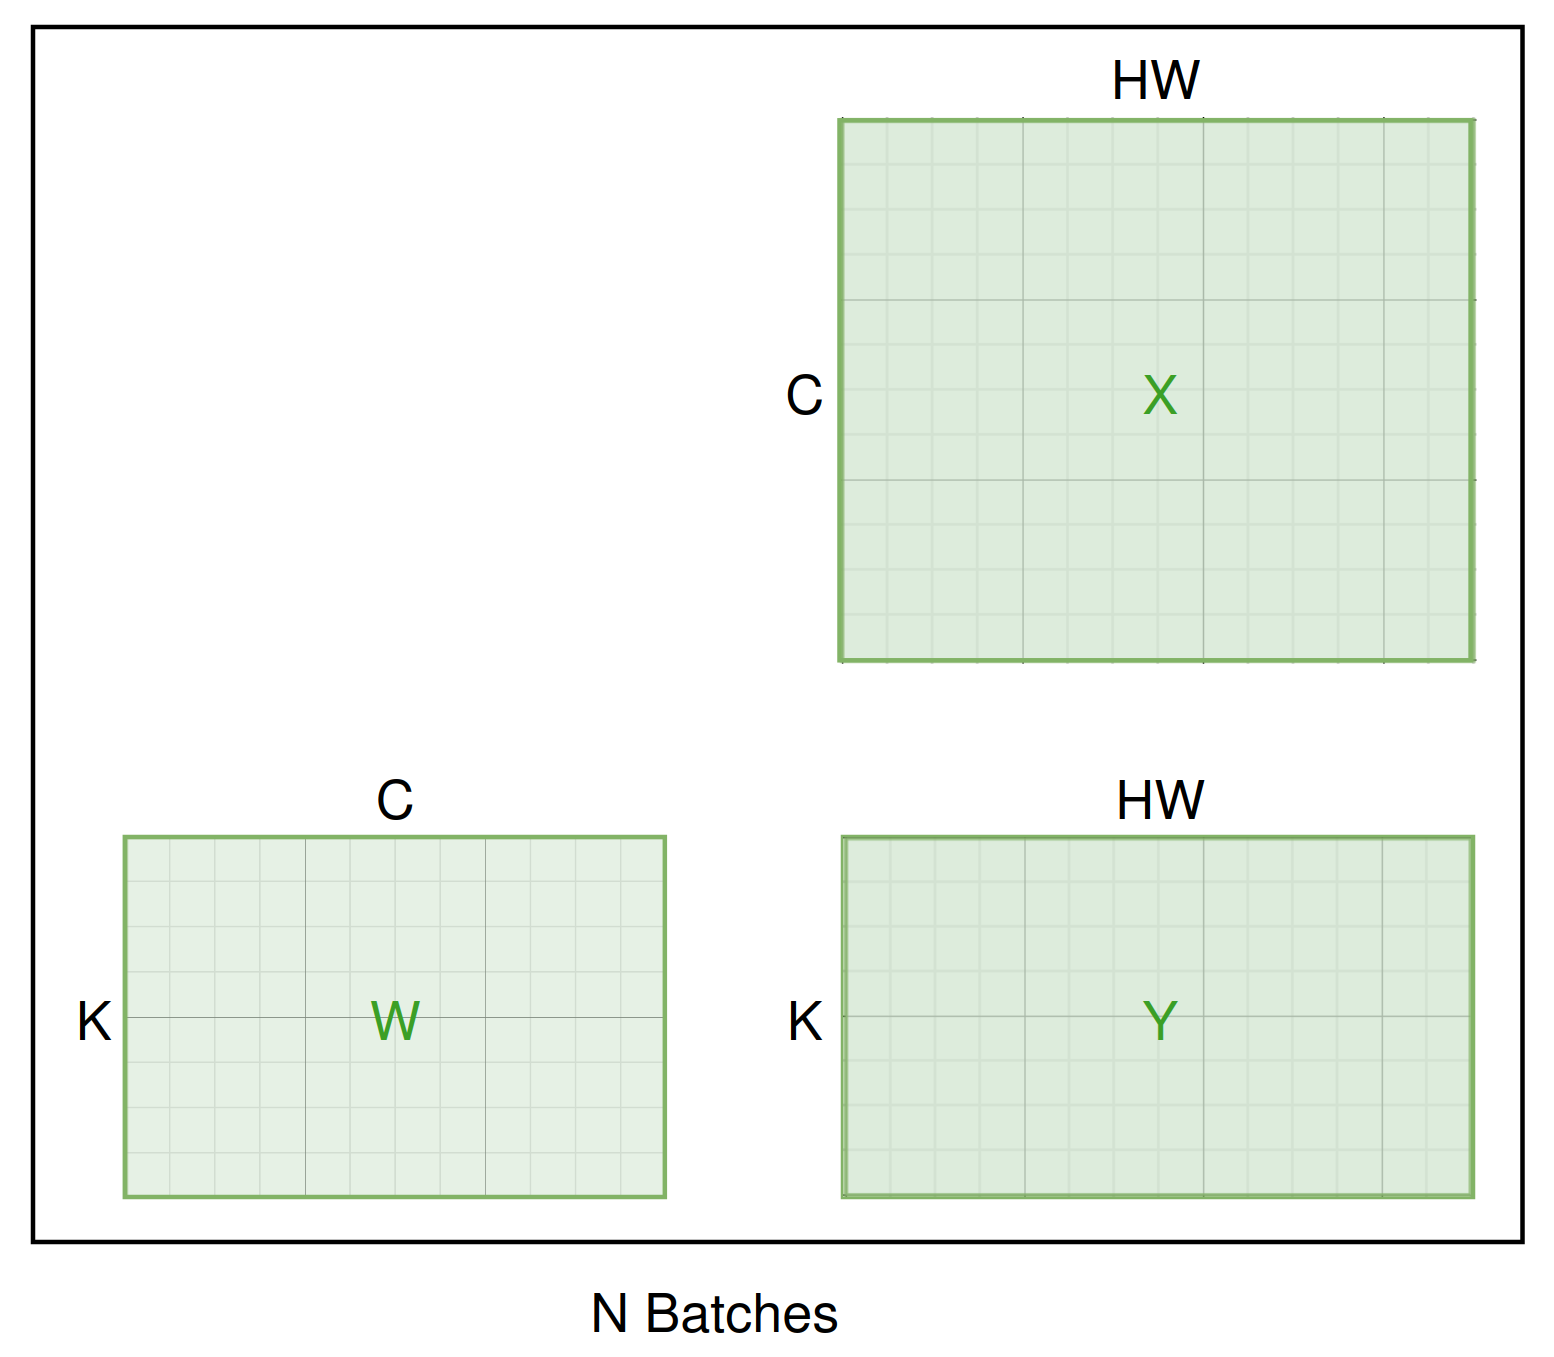
\includegraphics[width=0.8\textwidth]{src/images/1x1s0.png}
    \caption{Графическая схема преобразования свертки $1 \times 1$ с единичным шагом и нулевым дополнением в пакетное матричное умножение}
    \label{fig:1x1s0}
\end{figure}

На рисунке \ref{fig:1x1s0} показана визуализация данного преобразования, демонстрирующая эквивалентность операции свертки и пакетного матричного умножения.
Такое представление особенно полезно для оптимизации реализации, так как позволяет применять высокоэффективные алгоритмы матричного умножения, реализованные
в библиотеке CUTLASS.

\begin{figure}[h]
    \centering
    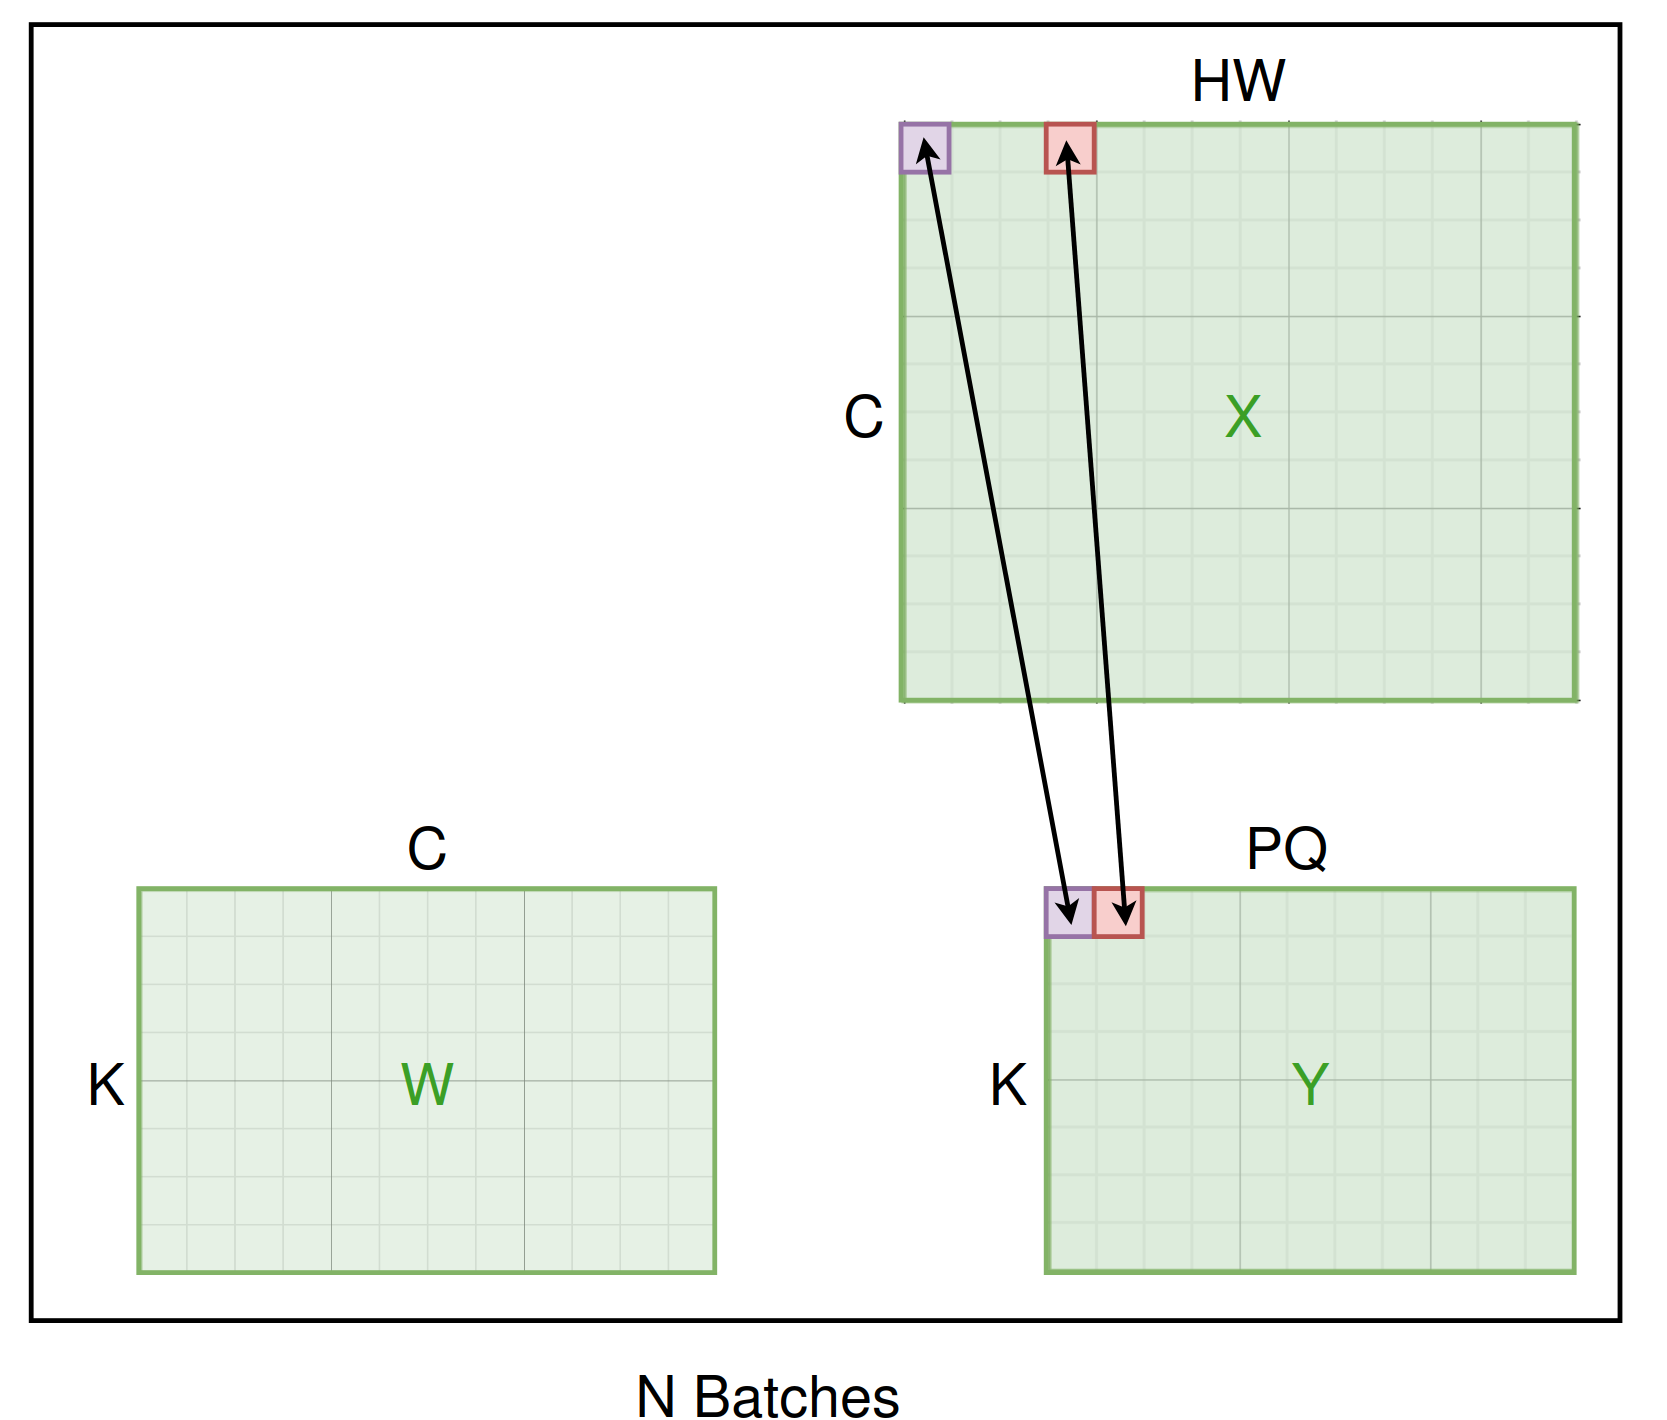
\includegraphics[width=0.8\textwidth]{src/images/1x1sn.png}
    \caption{Графическая схема преобразования свертки $1 \times 1$ с произвольным шагом и нулевым дополнением в пакетное матричное умножение}
    \label{fig:1x1sn}
\end{figure}

В случае свертки с произвольным шагом необходимо внести изменения в алгоритм пакетного матричного умножения.
Координаты входного тензора определяются соотношениями $\bar{h} = p \cdot s_h$ и $\bar{w} = q \cdot s_w$, где $s_h$ и $s_w$ — шаги свертки по
высоте и ширине соответственно.

Алгоритм преобразования включает следующие этапы:
\begin{enumerate}
    \item Введение составного индекса выходных пространственных координат: $pq = p \cdot Q + q$,
    \item Восстановление координат: $p = \lfloor pq / Q \rfloor$, $q = pq \bmod Q$,
    \item Вычисление соответствующих координат входного тензора: $\bar{h} = p \cdot s_h$, $\bar{w} = q \cdot s_w$.
\end{enumerate}

С математической точки зрения операция свертки записывается как

\begin{equation}
y[n, k, pq] = \sum_{c=0}^{C-1} w[k, c] \cdot x[n, c, \bar{h}\bar{w}],
\end{equation}

где индекс $\bar{h}\bar{w} = \bar{h} \cdot W + \bar{w}$ — линеаризованный индекс входного тензора.

Визуализация данного алгоритма приведена на рисунке \ref{fig:1x1sn}.

Оптимизированная реализация достигла 100 \% среднегеометрической производительности относительно cuDNN для
шага 1 и 85 \% для шага $>1$ (Рис. \ref{fig:conv1x1_res}):

\begin{figure}[htbp]
\centering
\begin{tikzpicture}
\begin{axis}[
    ybar=0pt,
    bar width=15pt,
    width=8cm,
    height=6cm,
    ylabel={Производительность относительно cuDNN},
    xlabel={Тип свёртки},
    symbolic x coords={k1x1s1x1, k1x1s2x2},
    xtick=data,
    xticklabel style={rotate=45, anchor=east},
    ymin=0,
    ymax=1.4,
    enlarge x limits=0.5,
    legend style={
        at={(0.5,1.03)},
        anchor=south,
        legend columns=-1,
    },
    nodes near coords,
    nodes near coords align={vertical},
    grid=major,
    grid style={dashed,gray!30}
]
\addplot+[
    style={fill=blue!40},
    every node near coord/.append style={
        font=\scriptsize,
        anchor=south
    }
] coordinates {(k1x1s1x1,1.0) (k1x1s2x2,0.85)};

\addplot+[
    style={fill=red!50},
    every node near coord/.append style={
        font=\scriptsize,
        anchor=south,
        xshift=4pt,
    }
] coordinates {(k1x1s1x1,0.56) (k1x1s2x2,0.62)};

\legend{Оптимизированный, Базовый}
\end{axis}
\end{tikzpicture}
\caption{Сравнение среднегеометрической производительности реализации свертки 1x1 для формата
NCHW относительно cuDNN: до оптимизации и после}
\label{fig:conv1x1_res}
\end{figure}

TBD;
	\clearpage

	\section{Заключение}
В данной дипломной работе была поставлена задача разработки высокопроизводительных библиотек машинного обучения cuBLAS и cuDNN,
предназначенных для выполнения матричного умножения, операций свёртки и пакетной нормализации. Основной целью работы стало создание
эффективных интерфейсов, которые могут быть использованы в нейронных сетях с фреймворком PyTorch, а также их тестирование на функциональном
и потактовом симуляторах, поддерживающих модель CUDA.

В процессе выполнения работы были решены ключевые задачи, включая разработку интерфейсов для основных операций, определение методологии тестирования
и оценка производительности разработанных библиотек. Проведённые исследования показали, что разработанные решения обеспечивают высокую производительность
и стабильность работы, соответствуя требованиям современных задач машинного обучения.

Разработана система тестирования, включающая функциональную проверку и оценку производительности на реальных устройствах NVIDIA Jetson и симуляторе gem5.
Проведено тестирование на широком спектре нейронных сетей (ResNet, EfficientNet, YOLOv11, UNET и др.), подтвердившее корректность работы библиотек в
реальных сценариях.

Разработаны оптимизированные версии операций \texttt{cublasLtMatmul}, \texttt{cudnnConvolutio\-nForward} и \texttt{cudnnBatchNormalizationForwardInference},
необходимые для запуска нейронных сетей, использующих фреймворк PyTorch. Для матричного умножения (\texttt{cublasL\-tMatmul}) реализован на базе библиотеки CUTLASS
и предложен алгоритм выбора оптимальных параметров, что позволило достичь 90 \% производительности эталонной реализации cuBLAS. Реализация пакетной нормализации
(\texttt{cudnnBatchNormalizationForwa\-rdInference}) продемонстрировала 99,7 \% производительности по сравнению с cuDNN для формата NCHW.
Операция свёртки (\texttt{cudnnConvolutionForward}) реализована для форматов NHWC и NCHW; для последнего дополнительно оптимизированы свёртки
с фильтром $1\times1$ как при единичном шаге свертки, так и при шаге, превышающем единицу. В результате оптимизаций достигнута производительность,
сопоставимая с cuDNN: 100\% для свертки $1\times1$ c шагом 1 и 85\% -- с шагом больше единицы.

Разработанные библиотеки cuBLAS и cuDNN обеспечивают высокую производительность, что делает их пригодными для использования в задачах машинного обучения на
GPGPU-ускорителях, поддерживающих модель CUDA. Результаты работы подтверждают возможность создания эффективных альтернатив проприетарным решениям NVIDIA с
сохранением функциональности и производительности.


	\clearpage

    \printbibliography

\end{document}
